\section{Word Embeddings}

\epigraph{
    Nets are for fish; once you get the fish you can forget the net.\\
    Words are for meaning; once you get the meaning you can forget the words.
}{Zhuangzi}

\newpage

\subsection{Introduzione}
Quando leggiamo un testo, noi esseri umani siamo dotati della capacità di coglierne un aspetto di significato. Questo implica che dietro alle parole che leggiamo si cela una rappresentazione semantica che vorremmo potenzialmente far apprendere anche alle macchine.  
Dal momento che le macchine parlano con la lingua dei numeri e, non come noi, con quella delle parole è stato necessario introdurre degli strumenti che vorrebbero in linea di principio assegnare ad ogni parola un numero rappresentatitivo di un singificato. Tale strumenti sono chiamati \emph{embeddings} e in questo capitolo, basandoci sul libro Speech and Language Processing di Stanford \cite{jm3}, si vedrà come vengono costruiti ed implementati per processare il testo.



\subsection{L'ipotesi distribuzionale}

Supponiamo di non conoscere il significato della parola \textit{ongchoi}, ma di 
incontrarla nei seguenti contesti:

\begin{enumerate}
    \item \textit{L'ongchoi è deliziosa saltata con aglio.}
    \item \textit{L'ongchoi è ottima servita con riso.}
    \item \textit{...foglie di ongchoi con salse salate...}
\end{enumerate}

Ora immaginiamo di aver già visto molte di queste parole-contesto in altri esempi, 
come:

\begin{enumerate}
   
    \item \textit{...gli spinaci saltati con aglio serviti sul riso...}
    \item \textit{...le coste, con i loro gambi e foglie, sono molto gustose...}
    \item \textit{...il cavolo riccio e altre verdure a foglia dal sapore salato...}
\end{enumerate} Il fatto che \textit{ongchoi} compaia insieme a parole come \textit{riso}, 
\textit{aglio}, \textit{deliziosa} e \textit{salata}, proprio come \textit{spinaci}, 
\textit{coste} o \textit{cavolo riccio}, suggerisce che l'ongchoi sia una 
\textbf{verdura a foglia} simile a queste altre verdure.
Questo è il principio dell'ipotesi distribuzionale per il quale la parola \textit{doctor-eye} o \textit{oculist} è probabile che la troviamo nello stesso contesto. 
\begin{notebox}
\textbf{Ipotesi Distribuzionale}
Si definisce ipotesi distribuzionale quella ipotesi per la quale parole simili compaiono in contesti simili.
\end{notebox}
Tale ipotesi suggerisce che il signficato delle parole venga appreso sulla base del contesto di dove queste appaiono. Se questa intuizione viene seguita allora può divenire possibile trovare una soluzione per assegnare dei numeri a delle parole sulla base della loro occorrenza dentro contesti. Prima di arrivare però a capire come costurire gli emebddings è necessario introdurre una ulteriore intuizione attibuita ad Osgood nel 1957.
\subsection{Ipotesi di Osgood}
Un contributo fondamentale alla rappresentazione del significato proviene dal 
lavoro di Osgood et al.\ (1957), che studiarono la componente affettiva delle parole. 
Osgood mostrò che i giudizi emotivi associati a una parola possono essere descritti 
lungo tre dimensioni principali:

\begin{enumerate}
    \item \textbf{Valenza}: quanto la parola è percepita come positiva o negativa.
    \item \textbf{Arousal}: quanto la parola induce attivazione emotiva.
    \item \textbf{Dominanza}: quanto la parola implica controllo o sottomissione.
\end{enumerate}

Ogni parola può quindi essere rappresentata come una tripla di valori numerici 
che ne definiscono la posizione in questo spazio tridimensionale. Ad esempio:

\[
\textit{heartbreak} \rightarrow [2.5,\ 5.7,\ 3.6]
\]

L’intuizione rivoluzionaria di Osgood è la seguente:


\begin{notebox}
\textbf{Ipotesi di Osgood}\\
Il significato di una parola può essere 
rappresentato come un vettore in uno spazio semantico.
\end{notebox}

Questa idea è stata la prima ad anticipare direttamente i moderni modelli di \textit{word embeddings}, in cui ogni 
parola è descritta come un punto in uno spazio multidimensionale corrispondente ad un singificato. 

\subsection{Verso i word embeddings}

L’unione dell’ipotesi distribuzionale e dell’ipotesi di Osgood ha aperto la strada
agli embeddings come modello fondamentale per la rappresentazione computazionale
del significato. Da un lato, l’ipotesi distribuzionale fornisce il principio secondo
cui il significato delle parole può essere inferito dai contesti in cui esse
compaiono; dall’altro, l’ipotesi di Osgood suggerisce che tale significato possa
essere rappresentato come un vettore numerico in uno spazio semantico.  
In questa sezione introduciamo i primi modelli di embedding basati su conteggi,
che costituiscono il punto di partenza storico e concettuale delle moderne
rappresentazioni distribuzionali. Per orientare il lettore, è utile chiarire fin da subito le principali tipologie
di embeddings che verranno introdotte nel seguito. In base alla natura della
rappresentazione prodotta, è possibile distinguere due grandi famiglie:
embeddings \textbf{statici} ed embeddings \textbf{dinamici}. 

\begin{notebox} \textbf{Embeddings statici}\ Si definisce statico un embedding in cui ogni parola del vocabolario è associata a un unico vettore pre-computato. Tale rappresentazione rimane invariata a prescindere dal contesto specifico in cui la parola appare. (Esempi: Matrici di co-occorrenza, Word2Vec, GloVe). \end{notebox}


Negli embeddings statici, a ciascun tipo di parola del vocabolario è associato un
unico vettore, indipendente dal contesto in cui la parola appare. Questa categoria
include sia gli embeddings distribuzionali basati su conteggi, come le matrici
termine--documento e termine--termine eventualmente ridotte tramite SVD, sia gli
embeddings predittivi appresi mediante modelli neurali, come Word2Vec. Gli embeddings dinamici, o contestuali, producono invece una rappresentazione
dipendente dal contesto: la stessa parola può essere associata a vettori diversi a
seconda della frase in cui compare. Tali rappresentazioni sono generate da modelli
di linguaggio neurali profondi, a partire da architetture ricorrenti fino ai
moderni modelli Transformer, come BERT.
\begin{notebox} \textbf{Embeddings dinamici (Contextual)}\ Si definisce dinamico un embedding in cui la rappresentazione vettoriale di una parola viene generata "al volo" in funzione dell'intera sequenza di input. La stessa parola riceve quindi vettori diversi a seconda del contesto semantico e sintattico circostante. (Esempi: ELMo, BERT, GPT). \end{notebox}



\begin{figure}[htbp] % h! può causare i problemi di underfull vbox, meglio htbp
\centering

\begin{forest}
  for tree={
    draw,
    rounded corners,
    fill=blue!5,
    align=center,
    font=\small,
    edge={->, thick},
    l sep=1.2cm,    
    s sep=0.5cm,    % Ridotto leggermente per farlo stare meglio nella pagina
    inner sep=6pt
  }
  [\textbf{Embeddings}
    [\textbf{Statici}
      [{\textbf{Count-based}\\(Term-Doc, Term-Term)}] % Graffe aggiunte qui
      [{\textbf{Predittivi neurali}\\(Word2Vec)}] % Graffe aggiunte qui
    ]
    [\textbf{Dinamici}
      [{\textbf{Modelli neurali profondi}\\(ELMo, BERT)}] % Graffe aggiunte qui
    ]
  ]
\end{forest}

\caption{Classificazione delle principali tipologie di embeddings trattate nel capitolo.}
\label{fig:classificazione_embeddings}
\end{figure}



\subsection{Embeddings count-based}

Il modo più semplice per costruire embeddings vettoriali delle parole è basato
sulla \textbf{matrice di co-occorrenza}, una struttura che codifica quante volte
determinati elementi linguistici compaiono insieme all’interno di un corpus.
Esistono diverse varianti di matrici di co-occorrenza; in questa sezione ne
introduciamo due fondamentali: la \emph{term-document matrix} e la
\emph{term-term matrix}. Iniziamo dal caso più semplice.
\subsubsection{Matrice termine-documento}

In una matrice termine-documento ogni riga rappresenta una parola del
vocabolario e ogni colonna rappresenta un documento appartenente a una collezione
di testi. Ogni cella della matrice contiene il numero di volte in cui la parola
associata alla riga compare nel documento associato alla colonna. Un esempio di term-document matrix è riportato nella Tabella
\ref{tab:term_document_shakespeare}, che mostra le occorrenze di quattro parole in
quattro opere di Shakespeare.

\begin{table}[h!]
\centering
\begin{tabular}{lcccc}
\hline
 & \textbf{As You Like It} & \textbf{Twelfth Night} & \textbf{Julius Caesar} & \textbf{Henry V} \\
\hline
battle & 1   & 0  & 7  & 13 \\
good   & 114 & 80 & 62 & 89 \\
fool   & 36  & 58 & 1  & 4  \\
wit    & 20  & 15 & 2  & 3  \\
\hline
\end{tabular}
\caption{Term-document matrix per quattro parole in quattro opere di Shakespeare.
Ogni cella contiene il numero di occorrenze della parola (riga) nel documento
(colonna). \cite{wang2024disentangledrepresentationlearning}}
\label{tab:term_document_shakespeare}
\end{table}

Questa matrice può essere interpretata in due modi distinti ma complementari.
Se si considerano le \textbf{colonne} della matrice, ciascun documento è
rappresentato come un vettore in uno spazio di dimensione $|V|$, dove $|V|$ è la
dimensione del vocabolario. In questo spazio, ogni asse corrisponde a una parola e
il valore lungo ciascuna dimensione indica la frequenza della parola nel
documento. Tale rappresentazione costituisce il fondamento del
\emph{vector space model} per il recupero dell’informazione, in cui documenti
simili sono associati a vettori geometricamente vicini. Alternativamente, se si considerano le \textbf{righe} della matrice, ogni parola
può essere interpretata come un vettore in uno spazio di dimensione pari al numero
di documenti. In questo caso, le dimensioni del vettore non corrispondono più a
parole, ma ai documenti del corpus, e il valore lungo ciascuna dimensione indica
quanto frequentemente la parola compare in ciascun documento. Questa seconda interpretazione è particolarmente rilevante dal punto di vista
semantico.

\begin{notebox}
\textbf{Interpretazione delle righe della matrice termine-documento}\\
Due parole risultano simili se presentano distribuzioni simili sui
documenti, ovvero se tendono a comparire negli stessi testi con frequenze
comparabili.
\end{notebox}

La term-document matrix fornisce quindi una prima, semplice forma di
\emph{embedding distribuzionale} delle parole, in cui il significato emerge dalla
loro distribuzione nei documenti del corpus.


\subsubsection{Matrice termine-termine}

Un’alternativa alla matrice termine--documento per la rappresentazione
distribuzionale delle parole è la matrice termine-termine, detta anche
\emph{word--word matrix} o \emph{term--context matrix}. In questo caso, le colonne
della matrice non sono più etichettate da documenti, bensì da parole del
vocabolario. La matrice ha quindi dimensionalità $|V| \times |V|$, dove $|V|$
indica la dimensione del vocabolario. In una matrice termine-termine, ogni riga rappresenta una \textbf{parola target}
e ogni colonna rappresenta una \textbf{parola di contesto}. Ciascuna cella
contiene il numero di volte in cui la parola di contesto compare nel contesto
della parola target all’interno di un corpus di addestramento. Formalmente, la
cella $M_{i,j}$ registra il numero di co-occorrenze tra la parola $w_i$ (target)
e la parola $w_j$ (contesto). Il concetto di \emph{contesto} può essere definito in diversi modi. Una possibilità
consiste nel considerare l’intero documento come contesto; tuttavia, nella pratica
è molto più comune utilizzare contesti locali, definiti tramite una
\textbf{finestra scorrevole} attorno alla parola target. Ad esempio, fissata una
finestra di ampiezza $\pm k$, una parola è considerata di contesto se compare entro
$k$ posizioni a sinistra o a destra della parola target nel testo. Considerando tutte le occorrenze di ciascuna parola nel corpus e contando le parole
che compaiono nelle rispettive finestre di contesto, è possibile costruire una
matrice di co-occorrenza parola--parola. La Tabella
\ref{tab:term_term_wikipedia} riporta un estratto reale di una matrice
termine--termine calcolata sul corpus Wikipedia, in cui sono mostrate quattro
parole target e alcune parole di contesto selezionate a scopo illustrativo
\cite{wang2024disentangledrepresentationlearning}.

\begin{table}[h!]
\centering
\begin{tabular}{lcccccc}
\hline
\textbf{Parola} & \textbf{aardvark} & \textbf{computer} & \textbf{data} & \textbf{result} & \textbf{pie} & \textbf{sugar} \\
\hline
cherry       & 0 & 2    & 8    & 9    & 442 & 25 \\
strawberry   & 0 & 0    & 0    & 1    & 60  & 19 \\
digital      & 0 & 1670 & 1683 & 85   & 5   & 4  \\
information  & 0 & 3325 & 3982 & 378  & 5   & 13 \\
\hline
\end{tabular}
\caption{Estratto di una matrice termine--termine calcolata sul corpus Wikipedia.
Ogni cella contiene il numero di co-occorrenze tra la parola target (riga) e la
parola di contesto (colonna) all’interno di una finestra di contesto locale
\cite{wang2024disentangledrepresentationlearning}.}
\label{tab:term_term_wikipedia}
\end{table}

In questa rappresentazione, ogni parola è associata a un vettore in uno spazio di
dimensione $|V|$, in cui ciascuna dimensione corrisponde a una parola di contesto.
Parole semanticamente simili tendono ad avere vettori simili, poiché compaiono in
contesti linguistici analoghi. Ad esempio, dalla Tabella
\ref{tab:term_term_wikipedia} si osserva che \textit{cherry} e \textit{strawberry}
co-occorrono frequentemente con parole come \textit{pie} e \textit{sugar},
suggerendo una forte affinità semantica, mentre \textit{digital} e
\textit{information} presentano distribuzioni simili rispetto a contesti come
\textit{computer} e \textit{data}.



\begin{notebox}
\textbf{Interpretazione della matrice termine--termine}\\
Due parole risultano semanticamente simili se presentano vettori di
co-occorrenza simili, ovvero se tendono a comparire negli stessi contesti
linguistici, anche nel caso in cui non compaiano mai direttamente insieme.
\end{notebox}
A questo punto abbiamo ottenuto una matrice termine-temrine,le cui colonne sono le parole di contesto, e i valori le co-occorrenze. Data $|V|$ la dimensione del vocabolario, tale matrice ha una dimensionalità
\begin{equation*}
    |V| \times |V|.
\end{equation*}
Si hanno tuttavia due problemi.
\begin{enumerate}
    \item Dal momento che ogni parole co-occorrerà solo con pochissime altre, \textit{la dimensionalità della matrice è enorme}.
    \item La maggior parte delle celle è nulla, e quindi \textit{i vettori sono estremamente sparsi}.
\end{enumerate}
Per affrontare i problemi legati all’elevata dimensionalità e alla 
natura estremamente sparsa della matrice termine-termine, ci sono diverse possibilità. Una di queste è la singular value decomposition in seugto descritta, e un'altra è quella di cambiare approccio e verrà presentata un'altra tipologia di embeddings basati su un altro paradigma di generazione diverso dal count-based che saranno successivamete presentati. 


\subsection{Riduzione dimensionale tramite SVD}
Un metodo per la riduzione della dimensionalità è la Singular Value Decomposition applicata alla word--context matrix. Sia $M \in \mathbb{R}^{|V| \times |V|}$ la word--context matrix, 
eventualmente pesata tramite tf-idf. 
La decomposizione ai valori singolari (Singular Value Decomposition, SVD) 
consente di fattorizzare $M$ come prodotto di tre matrici:
\[
M = U \Sigma V^\top
\]
dove $U$ e $V$ sono matrici ortogonali e $\Sigma$ è una matrice diagonale 
contenente i valori singolari ordinati in modo decrescente. Ogni valore singolare rappresenta l’importanza di una direzione latente 
nello spazio semantico. I valori singolari maggiori catturano le 
correlazioni più rilevanti tra parole e contesti, mentre quelli più piccoli 
tendono a modellare rumore o variazioni locali meno informative. Per ottenere una rappresentazione a dimensionalità ridotta, si considera 
una versione troncata della decomposizione, mantenendo solo i primi 
$k$ valori singolari:
\[
M \approx U_k \Sigma_k V_k^\top
\]
con $k \ll |V|$. Le righe della matrice $U_k \Sigma_k$ costituiscono una rappresentazione 
densa delle parole target in uno spazio latente di dimensione $k$. 
In questo nuovo spazio, ogni parola è descritta da un vettore 
a dimensionalità ridotta, in cui le correlazioni semantiche risultano 
più evidenti rispetto alla rappresentazione originale sparsa. È importante osservare che la riduzione dimensionale non elimina 
esplicitamente la sparsità della matrice originale, ma proietta le parole 
in uno spazio denso in cui le relazioni semantiche emergono in forma 
compressa e più robusta.

\subsection{Cosine Similarity}
Dal momento che i vettori di embeddings vivono in uno spazio vettoriale che è anche uno spazio semantico, è possibile calcolare l'affinità di significato che due vettori hanno tramine la cosine similarity.
La \textbf{cosine similarity} è una misura di similarità tra vettori che valuta 
il coseno dell’angolo compreso tra essi nello spazio vettoriale.  
Data la sua indipendenza dalla lunghezza dei vettori, risulta particolarmente 
adatta a confrontare vettori di frequenze o di pesi, come quelli derivati da 
matrici parola-contesto. Dati due vettori $u$ e $v$, la similarità coseno è definita come:

\begin{equation}
\text{cosine\_sim}(u, v) = 
\frac{u \cdot v}{\|u\| \, \|v\|}
= \frac{\sum_i u_i v_i}{\sqrt{\sum_i u_i^2} \, \sqrt{\sum_i v_i^2}}.
\end{equation}
Il valore risultante è compreso tra $-1$ e $1$:
\begin{itemize}
    \item $1$ indica che i vettori puntano nella stessa direzione (massima similarità),
    \item $0$ indica che sono ortogonali (nessuna similarità),
    \item valori negativi indicano direzioni opposte (molto raro nei contesti di NLP).
\end{itemize}
Nelle applicazioni di elaborazione del linguaggio naturale la cosine similarity è 
spesso preferita alla distanza Euclidea, perché ci interessa confrontare il 
\textit{pattern} delle co-occorrenze piuttosto che le loro magnitudini assolute.  
Ad esempio, due parole che co-occorrono con gli stessi termini di contesto, anche 
se con frequenze diverse, risulteranno comunque simili. La cosine similarity è quindi il principale strumento per valutare la similarità 
tra vettori distribuzionali e rappresenta un passaggio fondamentale prima di 
introdurre i modelli predittivi come Word2Vec e discendenti.


\subsection{Word2Vec: un approccio predittivo}
Sebbene i metodi basati su conteggi e la riduzione dimensionale tramite SVD permettano di ottenere rappresentazioni semanticamente dense, essi presentano limiti strutturali non trascurabili. Il calcolo della decomposizione ai valori singolari su matrici di co-occorrenza è computazionalmente oneroso, con una complessità che cresce sensibilmente rispetto alla dimensione del vocabolario, rendendo difficile la scalabilità su corpora massicci. 
Per superare queste criticità, Mikolov et al. (2013) hanno introdotto \textit{Word2Vec}, un framework basato su un paradigma radicalmente diverso: la \textbf{predizione}. Invece di riassumere statistiche globali, Word2Vec apprende gli embeddings processando il testo localmente. Lo spostamento di paradigma risiede nel fatto che, anziché contare le occorrenze totali, addestriamo un classificatore su un compito di \textbf{classificazione binaria}. Il modello deve rispondere alla domanda:

\begin{center}
\textit{``Data la parola target $w$ (es. \textit{albicocca}), qual è la probabilità che la parola candidata $c$ (es. \textit{marmellata}) compaia nel suo contesto?''}
\end{center}

In questo approccio, noto come \textbf{self-supervision}, il testo stesso fornisce le etichette: ogni parola $c$ che appare effettivamente vicino a $w$ nel corpus fornisce un esempio positivo (etichetta $1$). Al contrario, per addestrare il classificatore, il modello genera artificialmente degli esempi negativi campionando parole casuali dal vocabolario che non compaiono nel contesto di $w$.

\subsubsection{Il classificatore e la funzione sigmoide}

L'intuizione alla base del classificatore è che due parole siano semanticamente vicine se i loro vettori di embedding sono simili. Per misurare questa affinità, utilizziamo il \textbf{prodotto scalare} tra il vettore della parola target $\mathbf{w}$ e il vettore della parola di contesto $\mathbf{c}$:

\[
\text{Similarity}(w,c) \approx \mathbf{w} \cdot \mathbf{c}
\]

Poiché il prodotto scalare può assumere qualsiasi valore reale, utilizziamo la funzione \textbf{sigmoide} $\sigma(x)$ per mappare il risultato in una probabilità compresa tra $0$ e $1$:

\begin{equation}
\sigma(x) = \frac{1}{1 + e^{-x}}
\end{equation}

Il modello stima quindi la probabilità che la coppia $(w, c)$ sia un esempio positivo ($+$) come:
\begin{equation}
P(+ \mid w, c) = \sigma(\mathbf{w} \cdot \mathbf{c}) = \frac{1}{1 + e^{-\mathbf{w} \cdot \mathbf{c}}}
\end{equation}
Nel caso generale, data una parola target $w$ e un'intera finestra di $L$ parole di contesto $c_{1:L}$, il modello assume che le parole nel contesto siano indipendenti tra loro. La probabilità complessiva è dunque data dal prodotto delle probabilità individuali:
\begin{equation}
\log P(+ \mid w, c_{1:L}) = \sum_{i=1}^L \log \sigma(\mathbf{w} \cdot \mathbf{c}_i)
\end{equation}


\subsubsection{Perché due matrici? Il ruolo di $W$ e $C$}
Una caratteristica distintiva di Word2Vec è il mantenimento di \textbf{due rappresentazioni distinte} per ogni parola, organizzate in due matrici di pesi separate (Figura \ref{fig:skipgram_structure}). Una matrice $W$ relativa alle parole target che contiene i vettori utilizzati quando la parola è il centro della finestra, e una matrice $C$ che contiene i vettori utilizzati quando la parola appare nel contesto di un'altra o viene estratta come esempio negativo.


\begin{figure}[h!]
    \centering
    \includegraphics[width=0.7\textwidth]{pictures/embeddings_w2vec.png}
    \caption{Lo skip-gram apprende in totale due insiemi di embedding, uno per i target ($W$) e uno per i contesti ($C$), per un totale di $2|V|$ vettori. L’addestramento mira a massimizzare la probabilità che parole vicine nel testo abbiano vettori simili.}
    \label{fig:skipgram_structure}
\end{figure}
Sdoppiando le matrici, il modello garantisce la \textbf{stabilità dell'ottimizzazione}. Se usassimo un unico vettore $\mathbf{v}$, il modello cercherebbe di massimizzare il prodotto scalare $\mathbf{v} \cdot \mathbf{v}$ (auto-similarità), portando i valori a crescere all'infinito. Con due matrici, il modello apprende relazioni distribuzionali senza questo vincolo. Al termine, si utilizzano solitamente i vettori di $W$ o la media $W+C$.

\subsection{Proprietà semantiche degli embeddings}
L’apprendimento di questi vettori tramite il processo di ottimizzazione descritto non produce semplici sequenze numeriche prive di struttura, ma genera uno spazio geometrico capace di riflettere profonde relazioni linguistiche. La natura delle informazioni catturate da tali rappresentazioni dipende, in prima istanza, dalla configurazione della finestra di contesto, indicata come $L = 2m$, dove $m$ rappresenta il raggio d'azione a destra e a sinistra della parola target. Una finestra ristretta (con $m$ pari a 1 o 2) tende a privilegiare una similarità di tipo \textbf{sintattico}, raggruppando termini che condividono lo stesso ruolo grammaticale, come nel caso di verbi che occorrono in strutture frasali analoghe (ad esempio \textit{scrive}, \textit{dice} o \textit{risponde}). Al contrario, l’adozione di una finestra più ampia (con $m$ pari a 5 o più) sposta l’enfasi verso una similarità di tipo \textbf{topico} o tematico, associando parole che appartengono allo stesso ambito semantico, come \textit{ospedale}, \textit{ambulanza} e \textit{infermiere}, indipendentemente dalla loro funzione sintattica immediata. Questa capacità di astrazione permette agli embeddings densi di catturare efficacemente la similarità di secondo ordine.
\begin{notebox}
\textbf{Associazione paradigmatica (Similarità di secondo ordine)}\\
Due parole risultano vicine nello spazio vettoriale non perché compaiono necessariamente insieme nel testo (associazione sintagmatica di primo ordine), ma perché sono circondate da contesti simili.
\end{notebox}
Mentre l'ipotesi distribuzionale fornisce la base metodologica per inferire il significato, l'associazione paradigmatica ne rappresenta il successo fenomenologico più rilevante negli embeddings densi: la capacità di mappare vicini due termini che, pur non incontrandosi mai direttamente, svolgono la medesima funzione semantica nel discorso. 
Una delle manifestazioni più celebri di questa proprietà è la facoltà di supportare il ragionamento analogico attraverso il cosiddetto modello del parallelogramma. 
\begin{notebox}
\textbf{Modello del parallelogramma}\\
Il modello del parallelogramma postula che le relazioni semantiche tra coppie di parole siano codificate come differenze vettoriali costanti nello spazio degli embeddings. Data un'analogia del tipo ``$a$ sta ad $a^*$ come $b$ sta ad $b^*$'' (es. \textit{uomo} : \textit{donna} = \textit{re} : \textit{regina}), il termine incognito $b^*$ può essere approssimato tramite l'operazione algebrica:
\[ b^* \approx b - a + a^* \]
Geometricamente, ciò implica che il vettore che collega $a$ ad $a^*$ sia approssimativamente parallelo e di uguale lunghezza a quello che collega $b$ a $b^*$, formando idealmente i lati di un parallelogramma nello spazio vettoriale.
\end{notebox}
Tale regolarità permette di catturare relazioni grammaticali e semantiche complesse, dai passaggi di genere, come nella nota equazione $\text{king} - \text{man} + \text{woman} \approx \text{queen}$, fino ai rapporti geopolitici come $\text{Paris} - \text{France} + \text{Italy} \approx \text{Rome}$.
\begin{figure}[htbp]
\centering
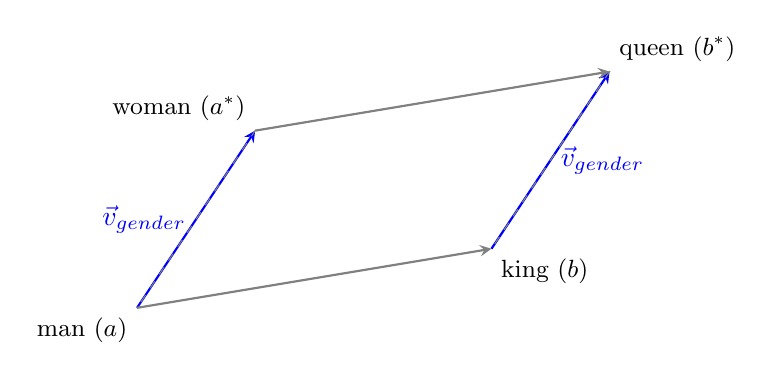
\begin{tikzpicture}[scale=1.5, >=stealth]
    % Coordinate dei punti
    \coordinate (man) at (0,0);
    \coordinate (woman) at (1,1.5);
    \coordinate (king) at (3,0.5);
    \coordinate (queen) at (4,2);

    % Vettori
    \draw[->, thick, blue] (man) -- (woman) node[midway, left] {$\vec{v}_{gender}$};
    \draw[->, thick, blue] (king) -- (queen) node[midway, right] {$\vec{v}_{gender}$};
    \draw[->, thick, gray] (man) -- (king) node[midway, below] {};
    \draw[->, thick, gray] (woman) -- (queen) node[midway, above] {};

    % Nodi (testo)
    \node[below left] at (man) {\small man ($a$)};
    \node[above left] at (woman) {\small woman ($a^*$)};
    \node[below right] at (king) {\small king ($b$)};
    \node[above right] at (queen) {\small queen ($b^*$)};

    % Linee tratteggiate per il parallelogramma
    \draw[dashed, gray] (man) -- (king) -- (queen) -- (woman) -- cycle;
\end{tikzpicture}
\caption{Rappresentazione geometrica del modello del parallelogramma applicato all'analogia di genere.}
\label{fig:parallelogramma}
\end{figure}
Da un punto di vista puramente geometrico, lo spazio degli embeddings è caratterizzato da proprietà di \textbf{parallelismo} e \textbf{ortogonalità}: mentre vettori paralleli indicano relazioni analoghe che si ripetono tra coppie diverse di parole, l’ortogonalità segnala l’indipendenza concettuale tra i termini. In sintesi, queste rappresentazioni apprese in modalità \textit{self-supervised} incorporano automaticamente una vasta gamma di informazioni sintattiche e semantiche, rendendo la scelta della dimensione del vettore e dell’ampiezza della finestra i parametri critici per determinare la qualità del risultato finale. Tuttavia, nonostante la loro straordinaria efficacia, questi modelli presentano un limite intrinseco dovuto alla loro natura \textbf{statica}: ogni parola del vocabolario è associata a un unico vettore che deve condensare in sé tutti i possibili sensi del termine, rendendo difficile la gestione della polisemia. Per superare questa rigidità e permettere alla rappresentazione di adattarsi dinamicamente al contesto specifico di ogni singola frase, la ricerca si è evoluta verso lo sviluppo degli embeddings dinamici.


\subsection{Embeddings dinamici}
Nelle sezioni precedenti abbiamo analizzato gli embeddings statici, i quali associano a ogni termine del vocabolario un unico vettore numerico invariante. Come evidenziato dai modelli classici come Word2Vec e GloVe, tale approccio permette di catturare relazioni semantiche globali, ma presenta un limite intrinseco: l'incapacità di gestire la polisemia e l'omonimia. In una rappresentazione statica, parole come \textit{spesso} (che può indicare una frequenza o uno spessore) o \textit{capo} (che può riferirsi a un indumento o a un superiore) sono costrette in un unico punto dello spazio vettoriale, che risulta essere una "media" forzata dei diversi sensi della parola.
Il passaggio verso gli \textbf{embeddings dinamici}, o contestuali, segna un cambiamento di paradigma fondamentale nel Natural Language Processing. In questo approccio, la rappresentazione di una parola non è più estratta da una tabella di ricerca (\textit{lookup table}) fissa, ma viene generata dinamicamente come funzione dell'intera sequenza di input. Ciò implica che la stessa parola riceverà vettori numerici differenti a seconda del contesto sintattico e semantico in cui appare.
\begin{notebox}
\textbf{Embeddings contestuali}\\
Data una sequenza di token $x_1, \dots, x_n$, un embedding contestuale è una rappresentazione vettoriale $h_i$ per il token $x_i$ tale che $h_i = f(x_i, C)$, dove $C$ rappresenta l'intera sequenza circostante (contesto). A differenza degli embeddings statici, $h_i$ rappresenta un'istanza specifica della parola (\textit{word instance}) e non la sua categoria astratta nel vocabolario (\textit{word type}).
\end{notebox}
Nella pratica, queste rappresentazioni emergono dagli stati interni di modelli di linguaggio neurali profondi. Mentre un embedding statico è un parametro del modello appreso durante l'addestramento e poi congelato, un embedding dinamico è il risultato computazionale dell'attivazione della rete durante la fase di inferenza. Per ottenere una rappresentazione robusta, è comune non limitarsi all'output dell'ultimo strato della rete neurale, ma combinare (ad esempio tramite media o concatenazione) le attivazioni provenienti da diversi livelli intermedi del modello, i quali catturano informazioni a diversi gradi di astrazione, dalla morfologia alla semantica complessa.
Questa flessibilità permette di risolvere il problema della polisemia: il modello "osserva" le parole circostanti e adatta il vettore della parola target per rifletterne il senso specifico in quel momento. Per comprendere come sia possibile trasformare una sequenza di parole in una sequenza di vettori così precisi, è necessario analizzare l'evoluzione delle architetture neurali, partendo dalle strutture progettate per gestire il tempo e la sequenzialità: le reti neurali ricorrenti.

\section{Reti Neurali Ricorrenti}
Il linguaggio è un fenomeno intrinsecamente temporale: la comprensione di una parola o di una frase dipende dalla sequenza di eventi acustici o testuali che l'hanno preceduta. I modelli precedentemente analizzati, come le reti feedforward a finestra fissa o gli embeddings statici, trattano l'input in modo simultaneo o limitato localmente, fallendo nel catturare dipendenze a lungo raggio.
Le Reti Neurali Ricorrenti (RNN), e in particolare le reti di Elman, introducono un meccanismo per gestire sequenze di lunghezza arbitraria tramite connessioni cicliche, permettendo al modello di mantenere una "memoria" del passato.

\begin{notebox}
\textbf{Rete Neurale Ricorrente}\\
Una RNN è una rete neurale in cui l'output di un neurone al tempo $t$ viene reimmesso come input allo stesso neurone al tempo $t+1$. Questo ciclo permette di modellare sistemi dinamici in cui l'output corrente dipende dall'intera storia degli input precedenti.
\end{notebox}

\noindent
Formalmente, data una sequenza di input rappresentata da vettori \textbf{one-hot} $\mathbf{x} = (\mathbf{x}_1, \dots, \mathbf{x}_T)$, dove ogni $\mathbf{x}_t \in \{0,1\}^{|V|}$ ha una dimensione pari alla cardinalità del vocabolario, il primo passaggio consiste nel recuperare l'embedding corrispondente. Sia $\mathbf{E} \in \mathbb{R}^{d \times |V|}$ la matrice di embedding, il vettore denso $\mathbf{e}_t$ al tempo $t$ è ottenuto tramite il prodotto:

\begin{equation}
\mathbf{e}_t = \mathbf{E}\mathbf{x}_t
\end{equation}

\noindent
Lo stato nascosto $\mathbf{h}_t$ viene calcolato combinando l'embedding corrente $\mathbf{e}_t$ con lo stato nascosto precedente $\mathbf{h}_{t-1}$:

\begin{equation}
\mathbf{h}_t = g(\mathbf{U}\mathbf{h}_{t-1} + \mathbf{W}\mathbf{e}_t + \mathbf{b})
\end{equation}

\begin{figure}[h!]
    \centering
    \includegraphics[width=\textwidth]{pictures/rnn.png}
    \caption{Illustrazione del funzionamento di una RNN. Ad ogni passo l'informazione contestuale viene consegnata a quello successivo.}
    \label{fig:rnn_flow}
\end{figure}

\noindent
Dove:
\begin{itemize}
    \item $\mathbf{W} \in \mathbb{R}^{d \times d}$ è la matrice dei pesi per l'input (embedding).
    \item $\mathbf{U} \in \mathbb{R}^{d \times d}$ è la matrice dei pesi ricorrenti.
    \item $\mathbf{b} \in \mathbb{R}^{d}$ è il vettore di bias.
    \item $g$ è una funzione di attivazione non lineare (solitamente $\tanh$ o ReLU).
\end{itemize}

\noindent
L'output della rete al tempo $t$, denotato con $\hat{\mathbf{y}}_t$, è una distribuzione di probabilità calcolata tramite la funzione \textbf{softmax} applicata a una proiezione dello stato nascosto:

\begin{equation}
\hat{\mathbf{y}}_t = \text{softmax}(\mathbf{V}\mathbf{h}_t + \mathbf{c})
\end{equation}

\noindent
Dove $\mathbf{V} \in \mathbb{R}^{|V| \times d}$ proietta lo stato nascosto nuovamente nello spazio del vocabolario per generare i punteggi (logits) per ogni parola.

\begin{figure}[htbp]
\centering
\includegraphics[width=\textwidth]{pictures/rnn_unrolled.png}
\caption{Rappresentazione srotolata (unrolled) di una RNN. Le frecce orizzontali mostrano il passaggio dello stato nascosto attraverso il tempo (pesi $\mathbf{U}$), mentre quelle verticali indicano l'elaborazione dell'input ($\mathbf{W}$) e la generazione dell'output ($\mathbf{V}$).}
\label{fig:rnn_unrolled}
\end{figure}

\subsection{RNN come Language Models}
I modelli di linguaggio hanno il compito di assegnare una probabilità a una sequenza di parole o, equivalentemente, di predire la parola successiva dato un contesto precedente. Per una sequenza di parole $w_{1:n}$, la probabilità congiunta può essere scomposta tramite la \textbf{regola della catena} (chain rule):

\begin{equation}
P(w_{1:n}) = \prod_{i=1}^{n} P(w_i \mid w_{1:i-1})
\end{equation}


Utilizzando una RNN, modelliamo questa probabilità condizionata assumendo che la dimensione dell'embedding $d_e$ e quella dello stato nascosto $d_h$ siano le stesse (dimensione del modello $d$). La probabilità che la parola successiva al tempo $t+1$ sia l'elemento $k$ del vocabolario è rappresentata dalla $k$-esima componente del vettore $\hat{\mathbf{y}}_t$:

\begin{equation}
P(w_{t+1} = k \mid w_1, \dots, w_t) = \hat{\mathbf{y}}_t[k]
\end{equation}

Di conseguenza, la probabilità dell'intera sequenza è definita come il prodotto delle probabilità dei termini corretti effettivamente osservati ad ogni passo temporale:

\begin{equation}
P(w_{1:n}) = \prod_{i=1}^{n} \hat{\mathbf{y}}_i[w_i]
\end{equation}

\subsubsection{Generaizone di Embeddings tramite RNN}
Questa architettura si presta a generare rappresentazioni delle parole, gli emebddings, capaci di adattarsi al contesto nel quale compaiono.
\begin{notebox}
\textbf{Embedding Contestuale nelle RNN}\\
In una RNN, il vettore $\mathbf{h}_t$ costituisce l'embedding contestuale della parola $w_t$. A differenza dell'embedding statico $\mathbf{e}_t$ (che è una semplice riga della matrice $\mathbf{E}$), il vettore $\mathbf{h}_t$ è dinamico: esso integra informazioni riguardanti l'intera storia della frase fino a quel momento.
\end{notebox}
Per estrarre questi embeddings da una RNN addestrata, si preleva lo stato $\mathbf{h}_t$ dal layer ricorrente. Questo vettore cattura sia la semantica intrinseca della parola corrente sia l'influenza sintattico-semantica del contesto precedente, risolvendo (in parte) i limiti degli embeddings statici nella gestione della polisemia.


\subsubsection{RNN Bidirezionali (Bi-RNN)}
Un limite intrinseco delle RNN analizzate finora è che lo stato nascosto $\mathbf{h}_t$ cattura esclusivamente le informazioni provenienti dal passato (contesto sinistro). Tuttavia, nel linguaggio naturale, il significato di una parola spesso dipende anche dalle parole che la seguono (contesto destro). 
Per ovviare a questo limite si utilizzano le RNN bidirezionali (Bi-RNN). L'idea alla base è quella di addestrare due reti distinte:
\begin{enumerate}
    \item Una RNN forward ($\overrightarrow{RNN}$) che processa la sequenza da sinistra a destra, generando una sequenza di stati $\overrightarrow{\mathbf{h}}_1, \dots, \overrightarrow{\mathbf{h}}_n$.
    \item Una RNN backward ($\overleftarrow{RNN}$) che processa la sequenza da destra a sinistra (dalla fine all'inizio), generando una sequenza di stati $\overleftarrow{\mathbf{h}}_n, \dots, \overleftarrow{\mathbf{h}}_1$.
\end{enumerate}

\begin{notebox}
\textbf{Embedding Contestuale Bidirezionale}\\
L'embedding contestuale finale per una parola $w_t$ si ottiene concatenando lo stato nascosto della rete forward con quello della rete backward:
\begin{equation}
\mathbf{h}_t^{bi} = [\overrightarrow{\mathbf{h}}_t \oplus \overleftarrow{\mathbf{h}}_t]
\end{equation}
In questo modo, il vettore risultante $\mathbf{h}_t^{bi}$ di dimensione $2d$ rappresenta la parola $w_t$ tenendo conto dell'intera frase circostante.
\end{notebox}

Questa rappresentazione è estremamente potente perché permette al modello di "sapere" cosa succederà in futuro mentre interpreta il presente, rendendo l'embedding molto più ricco per compiti come la traduzione automatica o il riconoscimento di entità nominate (NER).

\subsubsection{Il problema del Gradiente Svanente}
Nonostante la loro eleganza teorica, le RNN presentano dei limiti pratici significativi quando devono gestire sequenze molto lunghe. Il problema principale è noto come Vanishing Gradient.
Durante l'addestramento tramite l'algoritmo di \textit{Backpropagation Through Time} (BPTT), i gradienti vengono propagati all'indietro attraverso ogni passo temporale. Poiché il calcolo coinvolge moltiplicazioni ripetute della stessa matrice di pesi $\mathbf{U}$, se i valori di questa matrice sono piccoli, il segnale del gradiente tende a ridursi esponenzialmente man mano che ci si allontana nel passato.
\begin{enumerate}
    \item \textit{Perdita di dipendenze a lungo raggio:} Se una parola all'inizio della frase è cruciale per predire una parola alla fine (es. l'accordo di genere tra un soggetto e un participio molto distanti), la RNN "dimentica" l'informazione iniziale perché il gradiente non riesce a trasportare l'errore così indietro nel tempo.
    \item \textit{Instabilità:} Al contrario, se i pesi sono molto grandi, il gradiente può crescere a dismisura (\textit{Exploding Gradient}), rendendo l'addestramento instabile.
\end{enumerate}
Per risolvere l'incapacità delle RNN classiche di mantenere una memoria a lungo termine stabile, sono state introdotte architetture più sofisticate basate sul concetto di meccanismi di gating, come le LSTM (Long Short-Term Memory) che analizzeremo nella prossima sezione.




\subsection{LSTM: Long Short-Term Memory}

Nonostante l'accesso all'intera sequenza precedente, le RNN classiche faticano a gestire informazioni distanti dal punto corrente di elaborazione. Come osservato in \cite{jm3}, in una frase come:
\begin{quote}
    \textit{"The flights the airline was canceling were full."}
\end{quote}
Assegnare una probabilità corretta a \textit{were} è difficile perché il soggetto plurale \textit{flights} è distante, mentre il singolare \textit{airline} è più vicino nel contesto intermedio. Idealmente, una rete dovrebbe mantenere l'informazione del plurale fino a quando non è necessaria.
Questa incapacità delle RNN deriva da due problemi principali. La prima è la sovrapposizione di compiti: lo strato nascosto deve simultaneamente fornire informazioni per la decisione corrente e aggiornare/trasportare informazioni per il futuro.
Mentre la seconda è il già accennato problema del gradiente svanante (Vanishing Gradient): durante l'addestramento tramite \textit{backpropagation through time}, i gradienti vengono sottoposti a moltiplicazioni ripetute. Spesso questo processo porta i gradienti a zero, rendendo impossibile apprendere dipendenze a lungo raggio.
Le reti LSTM risolvono questi problemi dividendo la gestione del contesto in due compiti: rimuovere le informazioni non più necessarie e aggiungere quelle utili per il futuro. Lo fanno introducendo uno strato di contesto esplicito ($c_t$) e dei meccanismi di gating.
\subsection{Meccanismi di Gating}
I gate sono implementati tramite strati feedforward seguiti da una funzione sigmoide ($\sigma$) e da una moltiplicazione puntuale ($\odot$, o prodotto di Hadamard). La sigmoide spinge i valori verso 0 o 1, agendo come una maschera binaria: i valori vicino a 1 passano quasi invariati, quelli vicino a 0 vengono cancellati.
\begin{figure}[htbp]
    \centering
    \includegraphics[width=\textwidth]{pictures/lstm.png}
    \caption{Rappresentazione di una singola unità LSTM come grafo computazionale. Gli input consistono nell'input attuale $x_t$, lo stato nascosto precedente $h_{t-1}$ e il contesto precedente $c_{t-1}$. Gli output sono il nuovo stato nascosto $h_t$ e il contesto aggiornato $c_t$ \cite{jm3}.}
    \label{fig:lstm_unit}
\end{figure}
\subsection{Le equazioni del modello}
Seguendo fedelmente la formulazione di Jurafsky \& Martin \cite{jm3}, il calcolo per una singola unità LSTM all'istante $t$ è definito dalle seguenti operazioni:
\begin{enumerate}
    \item \textit{Forget Gate}. Determina quali informazioni eliminare dal contesto precedente $c_{t-1}$:
\begin{equation}
    f_t = \sigma (U_f h_{t-1} + W_f x_t)
\end{equation}
\begin{equation}
    k_t = c_{t-1} \odot f_t
\end{equation}
\item \textit{Add Gate}. Estrae le nuove informazioni e genera la maschera per decidere cosa aggiungere al contesto:
\begin{equation}
    g_t = \tanh(U_g h_{t-1} + W_g x_t)
\end{equation}
\begin{equation}
    i_t = \sigma (U_i h_{t-1} + W_i x_t)
\end{equation}
\begin{equation}
    j_t = g_t \odot i_t
\end{equation}
\item \textit{Aggiornamento del contesto}. Il nuovo vettore di contesto $c_t$ si ottiene sommando il contesto filtrato ($k_t$) e la nuova informazione selezionata ($j_t$):
\begin{equation}
    c_t = j_t + k_t
\end{equation}
\item \textit{Output Gate}. Decide quali informazioni del contesto devono essere esposte nello stato nascosto $h_t$:
\begin{equation}
    o_t = \sigma (U_o h_{t-1} + W_o x_t)
\end{equation}
\begin{equation}
    h_t = o_t \odot \tanh(c_t)
\end{equation}



\end{enumerate}








\subsubsection{Modularità ed Embeddings}
Lo stato nascosto $h_t$ fornisce l'output della LSTM a ogni passo temporale. Questo vettore costituisce l'embedding contestuale della parola, capace di integrare memorie a lungo termine. La complessità dell'unità è incapsulata, mantenendo una modularità che permette di sostituire le RNN con le LSTM in qualsiasi architettura complessa.


\section{Architettura Encoder-Decoder e limite del \textit{bottleneck}}
\label{sec:encoder_decoder_rnn}

Le LSTM (e, più in generale, le RNN) risolvono in modo parziale il problema del
\textit{vanishing gradient} e consentono di modellare dipendenze più lunghe rispetto alle
RNN ``classiche''. Tuttavia, quando il compito richiede di trasformare un'intera sequenza
in un'altra sequenza, come accade nella traduzione automatica, nel riassunto, o nella
risposta a domande in forma generativa, emerge un ulteriore vincolo strutturale.
In questi scenari non basta più produrre uno stato nascosto per ogni parola: occorre
un meccanismo che condensi l'informazione dell'input e la renda utilizzabile per
generare l'output.

\subsection{Il problema \textit{sequence-to-sequence}}
Consideriamo un input tokenizzato come
\[
X = (x_1, x_2, \dots, x_n),
\]
e un output
\[
Y = (y_1, y_2, \dots, y_m),
\]
con $m$ e $n$ in generale diversi. L'obiettivo è modellare la distribuzione condizionata
$P(Y\mid X)$, ovvero la probabilità di generare una sequenza $Y$ data la sequenza $X$.
Come in ogni modello linguistico autoregressivo, si applica la regola della catena:
\begin{equation}
P(Y\mid X) = \prod_{t=1}^{m} P(y_t \mid y_{<t}, X),
\label{eq:seq2seq_chain_rule}
\end{equation}
dove $y_{<t} = (y_1,\dots,y_{t-1})$.
L'architettura Encoder--Decoder affronta il problema separando comprensione
e generazione in due moduli distinti: un encoder che legge l'input e costruisce
una rappresentazione interna, e un decoder che, condizionato da tale rappresentazione,
genera l'output un token alla volta \cite{jm3}. Come si vede in Figura \ref{fig:fig:seq2seq_formal}, questa archiettura si scompone in due sotto architetture:
\begin{figure}[htbp]
    \centering
    \includegraphics[width=\textwidth]{pictures/seq2seq_formal.png}
    \caption{Schema formale dell'encoder--decoder ricorrente: l'encoder produce una sequenza di stati $h^{(e)}_1,\dots,h^{(e)}_n$ e il suo stato finale $h^{(e)}_n$ viene identificato con il vettore di contesto $c$, usato per inizializzare il decoder ($h^{(d)}_0$) e, nella variante mostrata, reso disponibile a ogni passo di decodifica. Questa dipendenza da un unico vettore di contesto anticipa il problema del \textit{bottleneck} discusso in seguito. Adattata da \cite{jm3}.}
    \label{fig:seq2seq_formal}
\end{figure}
\begin{enumerate}
    \item \textit{Encoder}. E' tipicamente una RNN/LSTM che processa l'input in ordine:
\begin{equation}
h_t^{(e)} = f_{\text{enc}}(x_t, h_{t-1}^{(e)}),
\qquad t = 1,\dots,n,
\label{eq:encoder_recurrence}
\end{equation}
dove $h_t^{(e)}\in\mathbb{R}^{d}$ è lo stato nascosto (o, nel caso LSTM, una funzione di stato
nascosto e memoria), e $f_{\text{enc}}$ indica la dinamica ricorrente. Nel modello ``classico'' Encoder-Decoder, l'intera sequenza viene riassunta in un singolo
vettore a dimensione fissa, spesso identificato con l'ultimo stato dell'encoder:
\begin{equation}
c \;\triangleq\; h_n^{(e)}.
\label{eq:context_vector}
\end{equation}
Questo vettore $c$ è chiamato \textit{context vector} (o \textit{sentence embedding}): dovrebbe contenere le informazioni necessarie per ricostruire,
tradurre o generare coerentemente l'output.

\item \textit{Decoder}. E' una seconda RNN/LSTM che definisce uno stato $h_t^{(d)}$ e produce, a ogni passo,
una distribuzione sul vocabolario tramite una proiezione e \texttt{softmax}:
\begin{align}
h_t^{(d)} &= f_{\text{dec}}(y_{t-1}, h_{t-1}^{(d)}, c), \label{eq:decoder_recurrence}\\
P(y_t \mid y_{<t}, X) &= \text{softmax}(W_o h_t^{(d)} + b_o). \label{eq:decoder_softmax}
\end{align}
In pratica, $c$ viene usato per inizializzare lo stato del decoder (o come input addizionale
a ciascun passo). Una scelta comune è
\begin{equation}
h_0^{(d)} = \phi(c),
\label{eq:decoder_init}
\end{equation}
dove $\phi$ è una trasformazione appresa (ad esempio lineare + non linearità).

\begin{notebox}
\textbf{Encoder-Decoder}\\
L'encoder trasforma una sequenza variabile $X$ in un vettore fisso $c$; il decoder usa $c$
come ``condizione'' per generare $Y$ in modo autoregressivo, implementando la
fattorizzazione in \eqref{eq:seq2seq_chain_rule}.
\end{notebox}

\end{enumerate}


\subsubsection{Il limite del \textit{bottleneck} informativo}
Il punto critico dell'architettura è evidente dalla definizione in \eqref{eq:context_vector}:
l'intera frase (potenzialmente lunga e ricca di dipendenze) viene compressa in un unico
vettore $c\in\mathbb{R}^d$. 


\begin{figure}[htbp]
    \centering
    \includegraphics[width=\textwidth]{pictures/bottleneck.png}
    \caption{Schema Encoder--Decoder: quando il contesto $c$ coincide con il solo stato nascosto finale dell'encoder,
    tutta l'informazione della sequenza sorgente deve attraversare un \emph{collo di bottiglia} rappresentazionale
    prima di essere utilizzata dal decoder.}
    \label{fig:encoder_decoder_bottleneck}
\end{figure}
Questa scelta introduce un vero e proprio
collo di bottiglia informativo:
\begin{enumerate}
    \item \textit{Compressione forzata.} All'aumentare della lunghezza e complessità dell'input,
    cresce la quantità di informazione che deve essere ``stipata'' in una dimensione fissa $d$.
    \item \textit{Sensibilità alla distanza.} Anche con LSTM, la rappresentazione finale tende a
    privilegiare informazione recente nella sequenza; dettagli importanti all'inizio possono
    attenuarsi o venire sovrascritti durante la ricorrenza.
    \item \textit{Difficoltà di allineamento.} In traduzione (e in molti task seq2seq) serve sapere
    \emph{quale parte} dell'input è rilevante per generare \emph{quel particolare} token di output.
    Un vettore unico $c$ non esplicita alcun allineamento fine-grained tra posizioni.
\end{enumerate}
Come illustrato in Figura~\ref{fig:encoder_decoder_bottleneck}, imporre che il contesto $c$
coincida con il solo stato finale dell’encoder costringe tutta l’informazione della frase sorgente
a passare attraverso un’unica rappresentazione a dimensione fissa, introducendo un collo di bottiglia. Questo limite è concettualmente analogo a quello discusso nel tuo Capitolo 2 sugli
autoencoders: anche lì un input complesso viene proiettato in uno spazio latente di
dimensione fissa, e il decoder tenta una ricostruzione a partire da tale compressione.
Nel caso seq2seq, però, la pressione sullo spazio latente è ancora più marcata, perché la
ricostruzione non riguarda ``lo stesso oggetto'' ma una sequenza diversa (es.\ tradotta),
che richiede sia contenuto semantico sia informazione strutturale \cite{jm3,jurafsky2024speech}.

\begin{notebox}
\textbf{Limite del bottleneck}\\
Nel modello Encoder-Decoder ricorrente, il contesto $c$ gioca il ruolo di uno \emph{spazio latente}
a dimensione fissa. Se $c$ non riesce a preservare le informazioni necessarie, il decoder è costretto
a generare una sequenza basandosi su una rappresentazione incompleta: questo è il \textit{bottleneck}.
\end{notebox}

\subsubsection{Soluzione al bottleneck: Meccanismo dell'attenzione}
\label{subsec:attention}
Il bottleneck dell'encoder--decoder ricorrente deriva dal vincolo \eqref{eq:context_vector}: l'unica informazione sull'input $X$ disponibile al decoder è un singolo vettore $c$, spesso identificato con lo stato finale dell'encoder. Questo implica che $c$ debba contenere tutta la semantica della frase sorgente e, per sequenze lunghe, le informazioni distanti (in particolare quelle all'inizio) possono risultare meno accessibili \cite{jm3}.
\begin{figure}[htbp]
\centering
\includegraphics[width=\textwidth]{pictures/attention_dynamic_context.png}
\caption{Nel meccanismo di attenzione, a ciascun passo di decodifica $i$ il decoder utilizza un contesto \emph{dinamico} $c_i$ (diverso per ogni token generato), calcolato come funzione di tutti gli stati nascosti dell'encoder. Adattata da \cite{jm3}.}
\label{fig:attention_dynamic_context}
\end{figure}
L'attenzione è una soluzione a questo collo di bottiglia: invece di obbligare il decoder a basarsi su un contesto statico, gli permette di ottenere informazione da tutti gli stati nascosti dell'encoder, selezionando dinamicamente la parte più rilevante dell'input a ogni passo di generazione (Figura~\ref{fig:attention_dynamic_context} e Figura~\ref{fig:attention_ci_computation}).
\begin{notebox}
\textbf{Meccanismo dell'attenzione}\\
Il meccanismo di attenzione sostituisce il contesto statico $c$ con un contesto dinamico $c_i$, calcolato come somma pesata degli stati dell'encoder. I pesi $\alpha_{ij}$ dipendono dallo stato del decoder e implementano un allineamento differenziabile tra posizioni dell'input e token generati in output, mitigando il \textit{bottleneck} dell'encoder--decoder ricorrente.
\end{notebox}
\begin{figure}[htbp]
\centering
\includegraphics[width=\textwidth]{pictures/attention_ci_computation.png}
\caption{Schema encoder--decoder con attenzione, focalizzato sul calcolo di $c_i$. Per ogni stato precedente del decoder $h^{(d)}_{i-1}$ si calcola un punteggio di rilevanza rispetto a ciascuno stato dell'encoder $h^{(e)}_j$; i punteggi vengono normalizzati in pesi $\alpha_{ij}$ e usati per ottenere $c_i$ come somma pesata degli stati dell'encoder. Adattata da \cite{jm3}.}
\label{fig:attention_ci_computation}
\end{figure}
Formalmente, sia $H = (h^{(e)}_1,\dots,h^{(e)}_n)$ la sequenza degli stati dell'encoder. L'attenzione introduce un vettore di contesto $c_i$ che viene ricalcolato a ogni passo di decodifica $i$ come funzione di tutti gli stati dell'encoder e dello stato precedente del decoder:
\[
c_i = f\!\big(h^{(e)}_{1:n},\, h^{(d)}_{i-1}\big).
\]
Il contesto $c_i$ entra direttamente nel calcolo dello stato nascosto del decoder, che diventa dipendente sia dalla storia del decoder sia dall'informazione selezionata dalla sorgente:
\begin{equation}
h^{(d)}_i = g\!\big(y_{i-1},\, h^{(d)}_{i-1},\, c_i\big).
\label{eq:decoder_with_attention_jm}
\end{equation}

Il primo passo per costruire $c_i$ consiste nel determinare quanto ciascuno stato dell'encoder $h^{(e)}_j$ sia rilevante per il passo corrente di decodifica. Per farlo si definisce una funzione di compatibilità (o \textit{alignment score}) tra lo stato precedente del decoder e lo stato $j$ dell'encoder:
\begin{equation}
\text{score}\!\big(h^{(d)}_{i-1}, h^{(e)}_{j}\big).
\label{eq:attention_score_general}
\end{equation}
La forma più semplice, detta dot-product attention, misura questa compatibilità come prodotto scalare:
\begin{equation}
\text{score}\!\big(h^{(d)}_{i-1}, h^{(e)}_{j}\big)=h^{(d)}_{i-1}\cdot h^{(e)}_{j}.
\label{eq:attention_dot_score}
\end{equation}
I punteggi così ottenuti vengono normalizzati con una softmax per produrre una distribuzione di pesi:
\begin{equation}
\alpha_{ij}=\frac{\exp\big(\text{score}(h^{(d)}_{i-1}, h^{(e)}_{j})\big)}{\sum_{k=1}^{n}\exp\big(\text{score}(h^{(d)}_{i-1}, h^{(e)}_{k})\big)}.
\label{eq:attention_weights_softmax}
\end{equation}
Per costruzione, $\alpha_{ij}\ge 0$ e $\sum_{j=1}^{n}\alpha_{ij}=1$. Il contesto dinamico si ottiene quindi come media pesata degli stati dell'encoder:
\begin{equation}
c_i=\sum_{j=1}^{n}\alpha_{ij}\,h^{(e)}_{j}.
\label{eq:attention_context_weighted_sum}
\end{equation}
In questo modo, pur mantenendo un vettore $c_i\in\mathbb{R}^d$ a dimensionalità fissa, il modello evita la compressione in un unico riassunto globale: l'informazione viene invece recuperata in modo selettivo dall'intera memoria dell'encoder e aggiornata passo per passo secondo le necessità del decoder \cite{jm3}.


\subsubsection{Verso i Transformer}
Una volta introdotta l'attenzione come accesso diretto a una memoria di stati, il passo successivo
(diventato centrale nella storia recente del NLP) è chiedersi se la ricorrenza sia ancora necessaria.
Se un modello può collegare direttamente, tramite pesi di attenzione, posizioni lontane della sequenza,
allora molte delle funzioni della memoria ricorrente possono essere replicate --- e spesso superate ---
da meccanismi puramente basati su attenzione. Questa osservazione è il punto di partenza dei
\textbf{Transformer}, in cui la dipendenza sequenziale della ricorrenza viene rimpiazzata da
\textbf{self-attention} e computazione parallelizzabile \cite{jm3}.

In sintesi, la traiettoria logica è:
\[
\text{RNN/LSTM} \;\rightarrow\; \text{Encoder--Decoder (bottleneck)} \;\rightarrow\;
\text{Attention (contesto dinamico)} \;\rightarrow\; \text{Transformer} \;\rightarrow\; \text{BERT}.
\]
Nella prossima sezione formalizziamo il meccanismo di attenzione e mostriamo come esso implementi,
in modo differenziabile, un allineamento tra posizioni dell'input e token generati in output.



\subsection{Il Transformer}
\label{sec:transformer}

\epigraph{
“The true art of memory is the art of attention.”
}{Samuel Johnson, \textit{The Idler}}

\begin{figure}[htbp]
\centering
\includegraphics[width=\textwidth]{pictures/transformer_overview.png}
\caption{Schema di un Transformer causale (left-to-right) per language modeling. Ogni token in input viene codificato (embedding del token e della posizione), processato da una pila di blocchi Transformer, e infine proiettato tramite una testa di language modeling per predire il token successivo.}
\label{fig:transformer_overview}
\end{figure}
Il Transformer è l'architettura di riferimento per la costruzione dei moderni modelli di linguaggio neurali. A differenza delle reti ricorrenti, esso non elabora la sequenza in modo strettamente sequenziale: la dipendenza tra token viene modellata tramite un meccanismo di attenzione applicato in parallelo alle posizioni della sequenza. Questa scelta consente di costruire rappresentazioni contestuali profonde, integrando informazione proveniente da token anche molto distanti, e rende il calcolo altamente parallelizzabile \cite{jm3}.
In questa sezione consideriamo, come caso base, il Transformer per language modeling autoregressivo (left-to-right), in cui dato un prefisso di token $(w_1,\dots,w_i)$ si stima una distribuzione di probabilità sul token successivo $w_{i+1}$. L'idea generale è che il modello produca, per ogni posizione $i$, un vettore contestuale che riassume ciò che è rilevante del contesto precedente per predire il prossimo token. La Figura~\ref{fig:transformer_overview} sintetizza la struttura, che può essere descritta tramite tre componenti principali.
\begin{enumerate}
    \item La prima componente è l'input encoding, che trasforma ciascun token $w_i$ in un vettore $x_i\in\mathbb{R}^{d}$ combinando un embedding lessicale con un'informazione di posizione. La sequenza di input viene così rappresentata come una matrice $X\in\mathbb{R}^{n\times d}$, dove $n$ è la lunghezza della finestra di contesto e $d$ è la dimensionalità del modello.
    \item La seconda componente è una pila di blocchi Transformer (stacked transformer blocks). Ogni blocco implementa una trasformazione che mappa la sequenza di vettori in input $(x_1,\dots,x_n)$ in una sequenza di vettori in output $(h_1,\dots,h_n)$ della stessa lunghezza e stessa dimensionalità. Il cuore di ciascun blocco è la multi-head self-attention, che costruisce una rappresentazione contestuale per ogni posizione pesando e combinando le rappresentazioni delle altre posizioni nel contesto. A questa si affiancano una rete feedforward punto-a-punto, connessioni residue e normalizzazioni, che stabilizzano e potenziano l'apprendimento \cite{jm3}. L'impilamento di molti blocchi consente al modello di costruire progressivamente rappresentazioni sempre più ricche, passando da segnali locali a dipendenze globali.
    \item La terza componente è la language modeling head, che a partire dal vettore prodotto per ciascuna posizione (tipicamente all'ultimo blocco) calcola dei punteggi sul vocabolario e, tramite softmax, una distribuzione di probabilità sul token successivo. In questa fase compare spesso una matrice di proiezione verso il vocabolario, concettualmente interpretabile come un'operazione inversa rispetto all'embedding (unembedding) \cite{jm3}.
\end{enumerate}
Nei paragrafi successivi entreremo nel dettaglio dei singoli elementi: prima formalizziamo la self-attention (Sezione~\ref{sec:self_attention}), poi descriviamo la struttura completa del blocco Transformer, la codifica posizionale e la testa di language modeling. Questa trattazione costituirà il passaggio naturale verso i modelli encoder bidirezionali, in particolare BERT, che utilizzano la stessa architettura di base ma con un regime di attenzione e un obiettivo di addestramento differenti \cite{jm3}.
%%%%%%%%%%%%%%%%%%%%%%%%%%%%%%%%%%
\subsection{Self-attention}
\label{subsec:self_attention}

\begin{figure}[htbp]
\centering
\includegraphics[width=\textwidth]{pictures/selfattn_alpha.png}
\caption{Esempio di distribuzione dei pesi di self-attention $\alpha$: per costruire una rappresentazione contestuale del token \emph{it} in uno strato superiore, il modello attribuisce peso maggiore ad alcuni token precedenti particolarmente informativi (ad es.\ \emph{chicken} e \emph{road}). In quel punto della sequenza, infatti, la coreferenza del pronome non è ancora disambiguata; è quindi plausibile che la rappresentazione di \emph{it} debba incorporare evidenza proveniente da entrambe le possibili entità.}
\label{fig:selfattn_alpha}
\end{figure}

\begin{figure}[htbp]
\centering
\includegraphics[width=\textwidth]{pictures/selfattn_flow.png}
\caption{Self-attention causale (left-to-right): in posizione $i$ il modello combina esclusivamente i token nelle posizioni $j\le i$ e, tramite mascheramento, non può incorporare informazione proveniente da posizioni future.}
\label{fig:selfattn_flow}
\end{figure}

\subsubsection{Motivazione: dalle rappresentazioni statiche alle rappresentazioni contestuali}
Negli \emph{embeddings statici} (ad es.\ Word2Vec o GloVe) a ciascun tipo lessicale del vocabolario viene associato un vettore fissato una volta per tutte: la parola assume dunque la medesima rappresentazione indipendentemente dall’enunciato in cui compare. Questo assunto, pur utile per catturare regolarità semantiche globali, risulta limitante quando il significato di un token dipende in modo cruciale dal contesto linguistico. In particolare, numerosi fenomeni del linguaggio naturale richiedono di mettere in relazione elementi anche molto distanti nella sequenza: (i) \emph{coreferenza} e risoluzione pronominale (un pronome può riferirsi a entità diverse), (ii) \emph{accordo morfosintattico} (ad esempio tra soggetto e verbo), (iii) \emph{disambiguazione del senso} (parole polisemiche che cambiano interpretazione in base al contesto), (iv) \emph{dipendenze sintattiche a lungo raggio}. 

L’obiettivo di un Transformer è costruire, strato dopo strato, una sequenza di \emph{rappresentazioni contestuali} (o \emph{contextual embeddings}), in cui il vettore associato a una posizione non descrive più soltanto il token in senso astratto, bensì la sua \emph{istanza} nel contesto specifico in cui occorre. Formalmente, a partire da una sequenza di input $X=(x_1,\dots,x_n)$, ogni strato produce una sequenza di output della stessa lunghezza, in cui ciascun elemento integra informazione selezionata dal contesto in modo differenziabile e appreso dai dati \cite{jm3}. In questo quadro, la \emph{self-attention} è il meccanismo centrale che determina \emph{da quali posizioni} recuperare informazione e \emph{con quale intensità}, producendo per ogni token una distribuzione di pesi sul contesto rilevante (Figura~\ref{fig:selfattn_alpha}).

\begin{notebox}
\textbf{Idea chiave}\\
La self-attention implementa un’operazione di \emph{retrieval differenziabile} sul contesto: per ciascuna posizione $i$, il modello calcola coefficienti $\alpha_{ij}$ che misurano la rilevanza delle posizioni $j$ (ammissibili) e costruisce una nuova rappresentazione come combinazione pesata delle informazioni recuperate. L’intero processo è appreso end-to-end durante l’addestramento \cite{jm3}.
\end{notebox}

\subsubsection{Self-attention causale: dominio informativo e vincolo di autoregressione}
Nel caso dei modelli autoregressivi (left-to-right), l’architettura deve essere coerente con la fattorizzazione causale della probabilità linguistica:
\[
P(w_{1:n})=\prod_{i=1}^{n}P(w_i\mid w_{1:i-1}).
\]
Di conseguenza, nel calcolo della rappresentazione della posizione $i$ non è consentito utilizzare token in posizioni future $j>i$, poiché ciò introdurrebbe una dipendenza non ammissibile (leakage di informazione) e renderebbe il modello incoerente con il compito di predizione del token successivo. In una self-attention \emph{causale}, pertanto, l’output in posizione $i$ dipende unicamente dal prefisso $(x_1,\dots,x_i)$:
\[
a_i = f(x_1,\dots,x_i),
\]
e l’intero strato realizza una mappatura parallela tra sequenze
\[
(x_1,\dots,x_n)\mapsto(a_1,\dots,a_n),
\]
in cui però, per ogni $i$, l’insieme delle posizioni consultabili è vincolato a $j\le i$ (Figura~\ref{fig:selfattn_flow}). Operativamente, tale vincolo viene implementato tramite una \emph{maschera causale} (o \emph{causal mask}) che annulla i contributi delle posizioni future prima della normalizzazione softmax.

\subsubsection{Intuizione: self-attention come combinazione pesata del contesto}
Per fissare l’idea, è utile introdurre una forma semplificata della self-attention: l’output $a_i$ in posizione $i$ può essere visto come una combinazione lineare delle rappresentazioni disponibili nel contesto ammissibile:
\begin{equation}
a_i=\sum_{j\le i}\alpha_{ij}x_j,
\label{eq:selfattn_weighted_sum}
\end{equation}
dove:
\begin{itemize}
    \item $\alpha_{ij}\in\mathbb{R}$ è un coefficiente scalare che misura il contributo della posizione $j$ all’aggiornamento della posizione $i$;
    \item nel caso standard, i pesi sono non-negativi e normalizzati (\emph{row-wise}) in modo da formare una distribuzione: $\alpha_{ij}\ge 0$ e $\sum_{j\le i}\alpha_{ij}=1$.
\end{itemize}
Questa formulazione mette in evidenza il punto essenziale: la rappresentazione contestuale di un token non è ottenuta “memorizzando” rigidamente il passato (come avviene nelle RNN), bensì \emph{selezionando} e \emph{aggregando} informazione da posizioni precedenti in modo adattivo. In altri termini, non tutti i token del prefisso sono ugualmente rilevanti: la self-attention apprende una strategia di selezione che enfatizza le parti del contesto più informative per il token corrente.

\subsubsection{Scaled dot-product attention: ruoli di query, key e value}
La formulazione effettivamente impiegata nei Transformer introduce tre proiezioni distinte della rappresentazione $x_i$ (tipicamente l’output dello strato precedente). Per ogni posizione $i$ si definiscono:
\begin{equation}
q_i=x_iW^Q,\qquad k_i=x_iW^K,\qquad v_i=x_iW^V,
\label{eq:qkv}
\end{equation}
dove $W^Q,W^K,W^V$ sono matrici di parametri apprendibili. L’interpretazione standard è la seguente \cite{jm3}:
\begin{itemize}
    \item $q_i$ (\emph{query}) codifica ciò che la posizione $i$ “richiede” al contesto, ossia quali caratteristiche cerca per aggiornare la propria rappresentazione;
    \item $k_j$ (\emph{key}) codifica ciò che la posizione $j$ “offre” come criterio di confronto rispetto alle query;
    \item $v_j$ (\emph{value}) contiene l’informazione effettiva che verrà aggregata se la posizione $j$ risulta rilevante.
\end{itemize}

\paragraph{Punteggi di compatibilità (scores).}
La rilevanza di una posizione $j$ per l’aggiornamento della posizione $i$ è stimata tramite un punteggio di compatibilità basato su prodotto scalare tra query e key:
\begin{equation}
\mathrm{score}(i,j)=\frac{q_i\cdot k_j}{\sqrt{d_k}},
\label{eq:score_scaled}
\end{equation}
dove $d_k$ è la dimensionalità dei vettori $q$ e $k$. Il fattore di scala $1/\sqrt{d_k}$ svolge un ruolo numerico fondamentale: senza scaling, all’aumentare di $d_k$ i prodotti scalari tendono ad assumere magnitudini elevate, e la softmax può saturare (distribuzioni eccessivamente “piccate”), riducendo l’efficacia del gradiente durante l’addestramento \cite{jm3}.

\paragraph{Normalizzazione tramite softmax e vincolo causale.}
I punteggi $\mathrm{score}(i,j)$ vengono convertiti in pesi di attenzione normalizzati tramite softmax sul contesto ammissibile:
\begin{equation}
\alpha_{ij}=\frac{\exp(\mathrm{score}(i,j))}{\sum_{t\le i}\exp(\mathrm{score}(i,t))}\qquad (j\le i).
\label{eq:alpha_softmax}
\end{equation}
Nel caso causale, la restrizione $j\le i$ si realizza introducendo una maschera $M$ tale che $M_{ij}=0$ se $j\le i$ e $M_{ij}=-\infty$ se $j>i$: i punteggi mascherati producono, dopo softmax, pesi nulli sulle posizioni future.

\paragraph{Aggregazione dei value e proiezione in output.}
L’output di una singola testa di attenzione (attention head) in posizione $i$ è quindi una somma pesata dei value:
\begin{equation}
\mathrm{head}_i=\sum_{j\le i}\alpha_{ij}v_j,\qquad a_i=\mathrm{head}_iW^O,
\label{eq:head_output}
\end{equation}
dove $W^O$ è una matrice di proiezione che riporta l’output alla dimensionalità del modello. In questa prospettiva, la self-attention può essere interpretata come un operatore che costruisce, per ciascuna posizione, una sintesi mirata del contesto, in cui la “selezione” è guidata dall’allineamento tra $q_i$ e le $k_j$ del prefisso.

\begin{figure}[htbp]
\centering
\includegraphics[width=\textwidth]{pictures/selfattn_head.png}
\caption{Calcolo di una singola testa di self-attention causale: (i) proiezioni in query/key/value; (ii) punteggi di compatibilità via dot-product scalato; (iii) normalizzazione in pesi $\alpha_{ij}$; (iv) somma pesata dei value per ottenere $\mathrm{head}_i$; (v) proiezione finale per ottenere $a_i$ in dimensione del modello.}
\label{fig:selfattn_head}
\end{figure}

\subsubsection{Forma matriciale e dimensioni (utile per l’implementazione)}
Sebbene la notazione per-indice chiarisca il significato, in un’implementazione la self-attention viene calcolata in forma matriciale. Indicando con $X\in\mathbb{R}^{n\times d}$ la matrice che raccoglie le rappresentazioni $x_i$ (una riga per token), si definiscono:
\[
Q=XW^Q,\qquad K=XW^K,\qquad V=XW^V.
\]
La matrice dei punteggi è $S=\frac{QK^\top}{\sqrt{d_k}}\in\mathbb{R}^{n\times n}$; applicando (eventualmente) una maschera causale $M$ si ottiene $S' = S+M$. La matrice dei pesi di attenzione si calcola applicando una softmax riga per riga:
\[
A=\mathrm{softmax}(S'),
\]
e infine l’output complessivo dello strato di attenzione (prima della proiezione finale) è:
\[
H = AV.
\]
Questa forma rende esplicito un aspetto computazionale cruciale: la self-attention confronta ogni posizione con (potenzialmente) tutte le altre posizioni del contesto, producendo una matrice $n\times n$; ciò implica un costo in tempo e memoria tipicamente quadratico in $n$ \cite{jm3}. Tale considerazione diventa rilevante quando si discute la scalabilità del Transformer a finestre di contesto molto ampie.

\subsubsection{Multi-head attention: pluralità di criteri di selezione}
Una singola testa di attenzione produce una sola distribuzione $\alpha_{i\cdot}$ e, di conseguenza, una sola combinazione pesata del contesto per ciascuna posizione. Tuttavia, le relazioni linguistiche di interesse sono molteplici (sintattiche, semantiche, morfologiche) e non è in generale desiderabile costringere un unico meccanismo a catturarle simultaneamente. Per questo motivo, i Transformer impiegano la \emph{multi-head attention}: si calcolano $A$ teste in parallelo, ciascuna con parametri distinti, e si combinano i risultati \cite{jm3}. Per ogni testa $c=1,\dots,A$:
\begin{equation}
q_i^{(c)}=x_iW^{Q}_{c},\qquad k_i^{(c)}=x_iW^{K}_{c},\qquad v_i^{(c)}=x_iW^{V}_{c},
\label{eq:qkv_multihead}
\end{equation}
da cui si ottengono i corrispondenti output $\mathrm{head}_i^{(c)}$. Gli output delle teste vengono quindi concatenati e proiettati per ripristinare la dimensionalità del modello:
\begin{equation}
a_i=\bigl(\mathrm{head}_i^{(1)}\oplus \mathrm{head}_i^{(2)}\oplus \dots \oplus \mathrm{head}_i^{(A)}\bigr)W^O.
\label{eq:multihead_concat}
\end{equation}
In termini dimensionali, se ciascuna testa produce un vettore in $\mathbb{R}^{d_v}$, la concatenazione produce un vettore in $\mathbb{R}^{A d_v}$; la matrice $W^O$ ha quindi forma $(A d_v)\times d$ e riporta l’output in $\mathbb{R}^{d}$, rendendo lo strato compatibile con connessioni residue e con l’impilamento di più blocchi. La conseguenza concettuale è che teste diverse possono apprendere criteri di selezione diversi e complementari (ad esempio, una testa può privilegiare dipendenze sintattiche, un’altra relazioni semantiche o segnali di coreferenza), aumentando la capacità espressiva del modello e la ricchezza delle rappresentazioni contestuali \cite{jm3}.

\begin{figure}[htbp]
\centering
\includegraphics[width=\textwidth]{pictures/multihead.png}
\caption{Multi-head attention: più teste calcolano in parallelo combinazioni pesate del contesto con parametri indipendenti; gli output vengono concatenati e proiettati per ottenere un vettore finale nella stessa dimensionalità dell’input.}
\label{fig:multihead}
\end{figure}

\subsubsection{Osservazione conclusiva: self-attention e contestualizzazione progressiva}
È opportuno sottolineare che la contestualizzazione non avviene in un singolo passaggio: in un Transformer profondo, la self-attention è applicata ripetutamente in una pila di blocchi. In ciascuno strato, i vettori $x_i$ (che possono essere visti come “stati” intermedi) vengono ricalibrati in funzione del contesto tramite pesi $\alpha_{ij}$ che dipendono a loro volta dalle rappresentazioni correnti. Ne risulta un processo di raffinamento progressivo, in cui gli strati inferiori tendono a catturare regolarità più locali, mentre quelli superiori integrano dipendenze più astratte e a più lungo raggio \cite{jm3}. In questo senso, la self-attention costituisce il principale meccanismo con cui il Transformer trasforma embeddings inizialmente non contestuali in rappresentazioni contestuali idonee alla predizione autoregressiva (o, in altre varianti, alla comprensione bidirezionale).

% ============================================================
% Sezione: Transformer Blocks (Jurafsky & Martin, Stanford)
% ============================================================

\subsection{Blocco Transformer}
\label{subsec:transformer_block}

Nella sezione precedente abbiamo visto come la \emph{self-attention} consenta a ciascun token
di costruire una rappresentazione contestuale combinando informazione da altre posizioni della
sequenza. Tuttavia, un Transformer reale non è composto da un singolo strato di attenzione:
la \textbf{unità modulare} che viene impilata molte volte per ottenere rappresentazioni sempre più
ricche è il \emph{blocco Transformer} (\textit{Transformer block}) \cite{jm3}. 
Lo scopo del blocco è duplice: (i) permettere alla self-attention di \emph{trasferire informazione}
tra token, e (ii) arricchire \emph{localmente} (token per token) la rappresentazione attraverso una
trasformazione non lineare, mantenendo al tempo stesso stabilità numerica e facilità di
ottimizzazione quando si impilano decine o centinaia di strati.

Un blocco Transformer contiene quattro componenti principali \cite{jm3}:
\begin{enumerate}
    \item \textbf{Multi-Head Self-Attention} (integra informazione tra posizioni diverse);
    \item \textbf{Feedforward Network} punto-a-punto (trasformazione non lineare applicata indipendentemente a ogni token);
    \item \textbf{Connessioni residue} (somma che preserva e propaga informazione lungo la profondità);
    \item \textbf{Layer Normalization} (normalizzazione che stabilizza l’addestramento).
\end{enumerate}

\begin{figure}[htbp]
    \centering
    % Salva l'immagine in: pictures/transformer_block_residual_stream.png
    \includegraphics[width=0.9\textwidth]{pictures/transformer_block.png}
    \caption{Architettura di un blocco Transformer nella variante \emph{prenorm} e interpretazione tramite
    \emph{residual stream}: ciascun modulo legge dallo stream del token e aggiunge il proprio output allo stesso stream
    tramite una somma residua \cite{jm3}.}
    \label{fig:transformer_block_residual_stream}
\end{figure}

\subsubsection{Input del blocco e informazione di posizione}
Sia $w_1,\dots,w_N$ una sequenza di token. All’ingresso di un blocco Transformer, ogni posizione $i$
è rappresentata da un vettore $x_i \in \mathbb{R}^d$. In generale, questo vettore non codifica soltanto
l’identità lessicale del token, ma anche \emph{la sua posizione} nella sequenza:
\begin{equation}
x_i = e(w_i) + p_i.
\label{eq:token_plus_positional}
\end{equation}
Qui $e(w_i)$ è l’embedding del token, mentre $p_i$ è l’\textbf{embedding posizionale}.
Quest’ultimo è necessario perché la self-attention, considerata da sola, è (in prima approssimazione)
\emph{invariante alle permutazioni}: senza un segnale di posizione, il modello non distinguerebbe una
sequenza da una sua riorganizzazione. Gli embeddings posizionali (sinusoidali o apprendibili)
iniettano quindi l’informazione d’ordine, rendendo possibile modellare fenomeni dipendenti dalla
struttura sequenziale (ad esempio dipendenze sintattiche) \cite{jm3}. 

\subsubsection{Residual stream: il flusso informativo del token}
Jurafsky \& Martin propongono una metafora utile per leggere il blocco Transformer: il
\textbf{residual stream} \cite{jm3}. L’idea è considerare, per ciascun token $i$, un unico flusso di vettori
in $\mathbb{R}^d$ che evolve attraversando i sottolivelli del blocco. Ogni sottolivello
(attenzione o feedforward) non \emph{sostituisce} la rappresentazione, ma calcola un aggiornamento che
viene \emph{aggiunto} allo stream tramite una connessione residua. Questo meccanismo ha due effetti
importanti:
\begin{itemize}
    \item preserva informazione utile anche quando il modello è molto profondo (il segnale può “scorrere” lungo le somme residue);
    \item facilita l’ottimizzazione, perché ogni sottolivello apprende una \emph{correzione} (residuo) rispetto a una rappresentazione già presente.
\end{itemize}

\subsubsection{Perché la LayerNorm (motivazione)}
Nel Transformer, le somme residue e l’impilamento di molti blocchi possono far crescere o oscillare
l’ampiezza delle attivazioni. La \textbf{layer normalization} serve a rendere l’addestramento più stabile
mantenendo i valori del vettore in un range numericamente ben condizionato per la discesa del gradiente
\cite{jm3}. È importante notare che la layer norm è applicata a \emph{un singolo token alla volta} (cioè
a un vettore in $\mathbb{R}^d$), non a un intero batch o a tutta la sequenza.

Dato $x \in \mathbb{R}^d$, si calcolano media e deviazione standard sulle sue componenti:
\begin{equation}
\mu = \frac{1}{d}\sum_{k=1}^{d} x_k,
\qquad
\sigma = \sqrt{\frac{1}{d}\sum_{k=1}^{d}(x_k - \mu)^2},
\end{equation}
e poi si normalizza introducendo due parametri apprendibili di scala e traslazione:
\begin{equation}
\text{LayerNorm}(x) = \gamma \frac{x-\mu}{\sigma} + \beta.
\label{eq:layernorm}
\end{equation}

\subsubsection{Feedforward network (ruolo)}
Accanto all’attenzione, ogni blocco include una rete \textbf{feedforward} applicata indipendentemente
a ciascun token. Mentre l’attenzione miscela informazione \emph{tra posizioni}, la FFN agisce come una
trasformazione non lineare \emph{locale} che aumenta la capacità espressiva del modello sul singolo token.
La forma standard è una rete a due strati:
\begin{equation}
\text{FFN}(x) = \text{ReLU}(x W_1 + b_1)\,W_2 + b_2,
\label{eq:ffn}
\end{equation}
con $W_1 \in \mathbb{R}^{d \times d_{ff}}$ e $W_2 \in \mathbb{R}^{d_{ff} \times d}$, e tipicamente $d_{ff} \gg d$
(ad esempio $d=512$, $d_{ff}=2048$ nel Transformer originale) \cite{jm3}.

\subsubsection{Equazioni del blocco (variante \emph{prenorm})}
Nella variante \textbf{prenorm} (Figura~\ref{fig:transformer_block_residual_stream}), la normalizzazione precede
attenzione e feedforward. Per chiarire la notazione, introduciamo una sequenza di vettori intermedi
$t_i^{(1)},\dots,t_i^{(5)} \in \mathbb{R}^d$ che rappresentano lo \emph{stato del residual stream} del token $i$
nei diversi passaggi interni al blocco. In altre parole, $t_i^{(k)}$ è semplicemente “ciò che scorre”
nello stream dopo il $k$-esimo sotto-passaggio del blocco \cite{jm3}.

Il blocco opera come segue:
\begin{align}
t_i^{(1)} &= \text{LayerNorm}(x_i), \\
t_i^{(2)} &= \text{MultiHeadAttention}\!\big(t_i^{(1)},\, t_1^{(1)},\dots,t_N^{(1)}\big), \\
t_i^{(3)} &= x_i + t_i^{(2)}, \\
t_i^{(4)} &= \text{LayerNorm}(t_i^{(3)}), \\
t_i^{(5)} &= \text{FFN}(t_i^{(4)}), \\
h_i &= t_i^{(3)} + t_i^{(5)}.
\label{eq:transformer_block_prenorm}
\end{align}
L’output $h_i \in \mathbb{R}^d$ ha la stessa dimensionalità dell’input $x_i$, il che rende possibile
impilare molti blocchi consecutivi senza cambiare forma ai vettori.

\subsubsection{L’attenzione come “movimento” di informazione tra stream}
Un fatto cruciale è che, all’interno del blocco, \textbf{solo la multi-head attention} accede a informazione
proveniente da altre posizioni della sequenza: FFN e LayerNorm operano localmente sul token $i$ \cite{jm3}.
Per questo motivo, nella metafora del residual stream, una testa di attenzione può essere interpretata come
un meccanismo che \emph{trasferisce} informazione dallo stream di un token $A$ a quello di un token $B$,
aggiornando la rappresentazione di $B$ con contenuto selezionato dal contesto.

\begin{figure}[htbp]
    \centering
    % Salva l'immagine in: pictures/attention_move_information.png
    \includegraphics[width=0.9\textwidth]{pictures/token_stream.png}
    \caption{Interpretazione della self-attention: una testa può spostare informazione dal residual stream del token $A$
    a quello del token $B$, integrando in $B$ contenuto recuperato da altre posizioni \cite{jm3}.}
    \label{fig:attention_moves_info}
\end{figure}

% ------------------------------------------------------------
% Nota pratica (paths):
% - Copia i file immagine nelle due posizioni indicate:
%   pictures/transformer_block_residual_stream.png
%   pictures/attention_move_information.png
% - Oppure modifica i path negli \includegraphics.
% ------------------------------------------------------------

% ============================================================
% Sezione 9.3 (Jurafsky & Martin): Parallelizzare con una sola matrice X
% ============================================================

\subsection{Parallelizzazione del calcolo con una singola matrice $X$}
\label{subsec:parallelizing_with_X}

Nelle sezioni precedenti abbiamo descritto la self-attention e il blocco Transformer
\emph{dal punto di vista di un singolo token} in posizione $i$, seguendo l’idea del residual stream.
Questa prospettiva è utile per capire \emph{che cosa} fa il modello, ma nasconde un fatto
computazionale cruciale: il calcolo della rappresentazione di ciascun token (attenzione,
layer norm e feedforward) è \emph{indipendente} da quello degli altri token, una volta fissata
la finestra di contesto. Per questo motivo l’intera computazione può essere eseguita in parallelo
con operazioni di algebra lineare, sfruttando routine ottimizzate di moltiplicazione tra matrici
\cite{jm3}.

\subsubsection{Impacchettare la sequenza in una matrice}
Sia $N$ la lunghezza della sequenza (window di contesto) e $d$ la dimensione del modello.
Raccogliamo i vettori di input $x_i \in \mathbb{R}^d$ in un’unica matrice:
\[
X \in \mathbb{R}^{N \times d},
\qquad
X =
\begin{bmatrix}
x_1^\top\\
\vdots\\
x_N^\top
\end{bmatrix}.
\]
Ogni riga di $X$ rappresenta quindi un token (token embedding + positional embedding, come discusso
nella sezione precedente), e lavorare in questa forma consente di calcolare in parallelo
tutte le rappresentazioni contestuali prodotte da un attention head o da un intero blocco Transformer.

\subsubsection{Self-attention in forma matriciale (una testa)}
Consideriamo una singola testa di attenzione. Invece di calcolare $q_i,k_i,v_i$ per ogni token
separatamente, proiettiamo l’intera matrice $X$ in tre matrici:
\begin{equation}
Q = XW^Q,\qquad K = XW^K,\qquad V = XW^V,
\label{eq:QKV_matrix}
\end{equation}
dove $W^Q,W^K \in \mathbb{R}^{d\times d_k}$ e $W^V \in \mathbb{R}^{d\times d_v}$.
Ne segue che $Q,K \in \mathbb{R}^{N\times d_k}$ e $V \in \mathbb{R}^{N\times d_v}$.

Il passo chiave è osservare che \emph{tutti} i confronti query--key $q_i\cdot k_j$ possono essere
ottenuti in un’unica moltiplicazione:
\[
S = QK^\top \in \mathbb{R}^{N\times N},
\]
dove la cella $S_{ij}$ contiene esattamente $q_i\cdot k_j$ (Figura~\ref{fig:qkt_full}).

\begin{figure}[htbp]
    \centering
    % Salva l'immagine in: pictures/qkt_full.png
    \includegraphics[width=0.9\textwidth]{pictures/qkt_full.png}
    \caption{La matrice $N\times N$ $QK^\top$: ogni cella contiene un confronto $q_i\cdot k_j$, calcolato
    simultaneamente con una singola moltiplicazione tra matrici \cite{jm3}.}
    \label{fig:qkt_full}
\end{figure}

Una volta ottenuti gli score, si applica lo scaling $1/\sqrt{d_k}$, la softmax riga-per-riga e
si combina il risultato con $V$:
\begin{equation}
\mathrm{head} = \mathrm{softmax}\!\Big(\mathrm{mask}\!\big(\tfrac{QK^\top}{\sqrt{d_k}}\big)\Big)\,V,
\label{eq:head_matrix}
\end{equation}
ottenendo una matrice $\mathrm{head}\in\mathbb{R}^{N\times d_v}$: una rappresentazione vettoriale
per ciascun token della sequenza, calcolata in parallelo \cite{jm3}.

\subsubsection{Mascheramento causale: eliminare il futuro}
La formulazione $QK^\top$ produce score tra ogni query $q_i$ e ogni key $k_j$, inclusi i casi $j>i$.
In un language model autoregressivo questo è inammissibile: per predire il token successivo, il modello
non deve accedere a token futuri. Per imporre il vincolo causale si applica una maschera triangolare superiore,
impostando gli elementi con $j>i$ a $-\infty$; la softmax li trasforma quindi in probabilità nulle \cite{jm3}:
\[
S' = S + M,
\quad\text{con}\quad
M_{ij}=
\begin{cases}
0 & \text{se } j\le i,\\
-\infty & \text{se } j>i.
\end{cases}
\]
Il risultato è illustrato in Figura~\ref{fig:qkt_masked}.

\begin{figure}[htbp]
    \centering
    % Salva l'immagine in: pictures/qkt_masked.png
    \includegraphics[width=0.9\textwidth]{pictures/qkt_masked.png}
    \caption{Mascheramento causale di $QK^\top$: la parte triangolare superiore (con $j>i$) è impostata a $-\infty$,
    così la softmax annulla i contributi dei token futuri \cite{jm3}.}
    \label{fig:qkt_masked}
\end{figure}

\subsubsection{Schema completo per una testa (in parallelo)}
La Figura~\ref{fig:single_head_parallel} riassume l’intero flusso computazionale in forma matriciale:
dalla costruzione di $Q,K,V$, al prodotto $QK^\top$, al mascheramento e alla combinazione pesata con $V$.

\begin{figure}[htbp]
    \centering
    % Salva l'immagine in: pictures/single_head_parallel.png
    \includegraphics[width=0.98\textwidth]{pictures/single_head_parallel.png}
    \caption{Computazione parallela di una singola testa di self-attention: (i) proiezioni $Q,K,V$ da $X$;
    (ii) calcolo di $QK^\top$; (iii) maschera causale; (iv) (softmax non mostrata nello schema); (v) somma pesata tramite $V$
    per ottenere l’output della testa \cite{jm3}.}
    \label{fig:single_head_parallel}
\end{figure}

\subsubsection{Costo computazionale e dipendenza quadratica}
Le Figure~\ref{fig:qkt_full} e~\ref{fig:qkt_masked} rendono evidente un limite strutturale:
ad ogni strato il modello deve calcolare confronti tra \emph{ogni coppia} di token nel contesto,
producendo una matrice $N\times N$. Ne segue che tempo e memoria della self-attention standard
crescono tipicamente come $\mathcal{O}(N^2)$ rispetto alla lunghezza del contesto \cite{jm3}.

\subsubsection{Multi-head attention in parallelo}
Nel caso multi-head, per ciascuna testa $c=1,\dots,A$ si usano matrici distinte
$W^Q_c,W^K_c,W^V_c$, ottenendo:
\begin{equation}
Q_c = XW^Q_c,\qquad K_c = XW^K_c,\qquad V_c = XW^V_c,
\label{eq:QKV_per_head}
\end{equation}
e la testa:
\[
\mathrm{head}_c = \mathrm{SelfAttention}(Q_c,K_c,V_c).
\]
Le $A$ uscite $\mathrm{head}_1,\dots,\mathrm{head}_A \in \mathbb{R}^{N\times d_v}$ vengono concatenate
lungo la dimensione delle feature e poi proiettate per ritornare alla dimensione del modello:
\begin{equation}
\mathrm{MultiHeadAttention}(X)=
\bigl(\mathrm{head}_1 \oplus \cdots \oplus \mathrm{head}_A\bigr)W^O,
\label{eq:multihead_parallel}
\end{equation}
dove $W^O \in \mathbb{R}^{(A d_v)\times d}$ e l’output complessivo ha forma $N\times d$ \cite{jm3}.

\subsubsection{Il blocco Transformer in forma parallela}
Infine, anche l’intero blocco Transformer può essere scritto in modo compatto usando matrici.
Nella variante \emph{prenorm} \cite{jm3}:
\begin{align}
O &= X + \mathrm{MultiHeadAttention}(\mathrm{LayerNorm}(X)),
\label{eq:block_parallel_O}\\
H &= O + \mathrm{FFN}(\mathrm{LayerNorm}(O)).
\label{eq:block_parallel_H}
\end{align}
Qui $X$ è l’input del blocco (per il primo strato è la matrice di embedding iniziale, per gli strati successivi
è l’output $H$ dello strato precedente), mentre $H\in\mathbb{R}^{N\times d}$ è l’output del blocco.
Notazione come $\mathrm{FFN}(O)$ indica che \emph{la stessa} rete feedforward viene applicata in parallelo
a ciascuna riga (cioè a ciascun token) della matrice \cite{jm3}.

% ------------------------------------------------------------
% Nota pratica (paths immagini):
% Copia/salva le tre figure che mi hai dato in:
%   pictures/qkt_full.png
%   pictures/qkt_masked.png
%   pictures/single_head_parallel.png
% (oppure modifica i path negli \includegraphics).
% ------------------------------------------------------------

% ============================================================
% 9.4 — The input: embeddings for token and position (JM3)
% ============================================================

\subsection{L'input del Transformer: embeddings di token e di posizione}
\label{subsec:input_token_position_embeddings}

Nella sezione precedente abbiamo visto come l’intera computazione di self-attention
possa essere espressa e parallelizzata tramite una singola matrice di input
$X \in \mathbb{R}^{N\times d}$, dove $N$ è la lunghezza del contesto e $d$ la dimensione del modello.
Resta ora da chiarire \textbf{da dove provenga} questa matrice $X$, ovvero come una sequenza discreta
di token venga trasformata in una sequenza di vettori densi adatti a essere processati
dai blocchi Transformer \cite{jm3}.

L’idea fondamentale è che l’input venga ottenuto combinando due sorgenti di informazione:
\begin{enumerate}
    \item un \textbf{embedding lessicale} (token embedding), che codifica l’identità del token;
    \item un \textbf{embedding posizionale} (positional embedding), che codifica la posizione del token nella sequenza.
\end{enumerate}
La loro somma produce una rappresentazione composita che costituisce l’input effettivo del Transformer.

\subsubsection{Token embeddings e matrice di embedding}
Sia $V$ il vocabolario dei token (tipicamente ottenuto tramite BPE o SentencePiece).
Una volta tokenizzato l’input, ogni token viene rappresentato da un indice intero $w_i \in \{1,\dots,|V|\}$.
Gli embeddings iniziali dei token sono memorizzati in una matrice:
\[
E \in \mathbb{R}^{|V|\times d},
\]
dove la riga $E[w_i]$ (di dimensione $d$) rappresenta l’embedding del token con indice $w_i$ \cite{jm3}.
Dunque, dato un token in posizione $i$, il suo embedding lessicale è:
\[
e(w_i) = E[w_i] \in \mathbb{R}^{d}.
\]

\paragraph{Selezione via one-hot (interpretazione equivalente).}
Un modo alternativo (concettuale) per vedere la selezione dell’embedding consiste nel rappresentare
il token con un vettore one-hot $\mathbf{o}(w_i)\in\{0,1\}^{|V|}$, con un unico 1 nella posizione $w_i$.
Moltiplicando $\mathbf{o}(w_i)$ per la matrice $E$ si “estrae” la riga corrispondente:
\[
\mathbf{o}(w_i)^\top E = E[w_i].
\]
La Figura~\ref{fig:select_single_embedding} illustra graficamente questa interpretazione \cite{jm3}.

\begin{figure}[htbp]
    \centering
    % Salva l'immagine in: pictures/select_single_embedding.png
    \includegraphics[width=0.88\textwidth]{pictures/select_single_embedding.png}
    \caption{Selezione dell’embedding del token $w_i$ a partire dalla matrice $E$ mediante un vettore one-hot:
    il prodotto \(\mathbf{o}(w_i)^\top E\) restituisce la riga \(E[w_i]\) \cite{jm3}.}
    \label{fig:select_single_embedding}
\end{figure}

\paragraph{Dalla sequenza alla matrice.}
Estendendo l’idea, l’intera sequenza di $N$ token può essere rappresentata come una matrice di one-hot
$O \in \{0,1\}^{N\times |V|}$ (una riga per posizione). Il prodotto:
\[
OE \in \mathbb{R}^{N\times d}
\]
restituisce una matrice che contiene, riga per riga, gli embeddings lessicali della sequenza
(Figura~\ref{fig:select_sequence_embedding}) \cite{jm3}. Nella pratica si usa indicizzazione diretta
sulle righe di $E$ (più efficiente), ma l’interpretazione one-hot chiarisce perché l’operazione sia
lineare e parallelizzabile.

\begin{figure}[htbp]
    \centering
    % Salva l'immagine in: pictures/select_sequence_embedding.png
    \includegraphics[width=0.88\textwidth]{pictures/select_sequence_embedding.png}
    \caption{Selezione degli embeddings per un’intera sequenza: una matrice di one-hot \(O\) moltiplicata per
    \(E\) produce una matrice \(N\times d\) contenente gli embeddings lessicali della finestra di contesto \cite{jm3}.}
    \label{fig:select_sequence_embedding}
\end{figure}

\subsubsection{Perché servono gli embeddings posizionali}
Gli embeddings di token, da soli, \emph{non} codificano la posizione: il token \textit{bill} ha lo stesso
vettore sia che compaia all’inizio sia che compaia alla fine della frase. Tuttavia, nei modelli di linguaggio
l’ordine è essenziale: molte regolarità sintattiche e semantiche dipendono dalla struttura sequenziale.
Inoltre, la self-attention confronta token tramite similarità tra query e key; senza un segnale di posizione,
il modello avrebbe difficoltà a distinguere configurazioni che differiscono solo per permutazione \cite{jm3}.
Per questo motivo, al token embedding si affianca un embedding di posizione.

\subsubsection{Posizione assoluta e composizione dell’input}
La soluzione più semplice è usare \textbf{posizione assoluta}: si associa a ogni posizione $i$ un vettore
$p_i \in \mathbb{R}^d$, apprendibile durante l’addestramento, raccolto in una matrice:
\[
E_{\text{pos}} \in \mathbb{R}^{N\times d},
\qquad p_i = E_{\text{pos}}[i].
\]
L’input finale per il token in posizione $i$ è la somma:
\begin{equation}
x_i = e(w_i) + p_i,
\label{eq:composite_embedding}
\end{equation}
e impilando tutti i vettori si ottiene:
\[
X =
\begin{bmatrix}
x_1^\top\\
\vdots\\
x_N^\top
\end{bmatrix}
\in \mathbb{R}^{N\times d}.
\]
In altre parole, \textbf{$X$ è una matrice di embeddings compositi} (token + posizione), che costituisce
l’input al primo blocco Transformer \cite{jm3}. La Figura~\ref{fig:token_plus_position} visualizza l’operazione:
a ogni token embedding viene sommato il corrispondente embedding di posizione, producendo un vettore della stessa dimensionalità.

\begin{figure}[htbp]
    \centering
    % Salva l'immagine in: pictures/token_plus_position.png
    \includegraphics[width=0.92\textwidth]{pictures/token_plus_position.png}
    \caption{Composizione dell’input: l’embedding del token viene sommato all’embedding della posizione assoluta,
    producendo un vettore di input \(x_i\) in \(\mathbb{R}^d\). L’insieme dei vettori forma la matrice \(X \in \mathbb{R}^{N\times d}\) \cite{jm3}.}
    \label{fig:token_plus_position}
\end{figure}

\begin{notebox}
\textbf{Input del Transformer}\\
La matrice \(X\in\mathbb{R}^{N\times d}\) contiene una riga per token, ed è costruita come
\(x_i = E[w_i] + E_{\text{pos}}[i]\). I blocchi Transformer trasformano poi \(X\) in rappresentazioni
contestuali sempre più ricche, mantenendo costante la dimensionalità \(d\) per poter essere impilati.
\end{notebox}

% ============================================================
% Sezione successiva (logica): limiti della posizione assoluta e alternative
% ============================================================

\subsection{Limiti della posizione assoluta e alternative: sinusoidale e posizione relativa}
\label{subsec:positional_alternatives}

L’approccio a posizione assoluta è concettualmente semplice e funziona bene, ma presenta un potenziale
limite: le posizioni più “lontane” (verso la massima lunghezza $N$) possono essere viste meno spesso
durante l’addestramento, e quindi i relativi embeddings $p_i$ rischiano di essere appresi in modo meno robusto
e di generalizzare peggio \cite{jm3}. Per mitigare questo problema, sono state proposte due famiglie di alternative.

\paragraph{Embeddings posizionali sinusoidali.}
Una prima alternativa consiste nel sostituire i vettori posizionali appresi con una funzione deterministica
che mappa l’indice di posizione $i$ in un vettore reale, ad esempio usando combinazioni di seni e coseni a
frequenze diverse (come nel Transformer originale). Questa scelta ha due vantaggi: (i) non richiede parametri
addizionali per ogni posizione, e (ii) introduce regolarità geometriche che riflettono relazioni tra posizioni,
rendendo più naturale rappresentare che posizioni vicine (es.\ $i$ e $i\!+\!1$) siano più correlate di posizioni
molto distanti \cite{jm3}.

\paragraph{Posizione relativa.}
Una seconda linea di lavoro, più espressiva, mira a modellare non la posizione assoluta di un token,
ma la sua \textbf{posizione relativa} rispetto agli altri token. In questo caso, l’informazione posizionale
viene spesso incorporata direttamente nel meccanismo di attenzione a ogni strato, in modo che i pesi di attenzione
possano dipendere esplicitamente dalla distanza (o dall’offset) tra le posizioni \cite{jm3}. 
Questa idea è particolarmente utile quando si vogliono gestire sequenze molto lunghe e favorire la generalizzazione
oltre le lunghezze viste in training.

\medskip
Queste tecniche completano la definizione dell’input del Transformer: una volta costruita la matrice \(X\),
il modello può applicare in parallelo i blocchi Transformer e, alla fine, utilizzare le rappresentazioni prodotte
per il compito di language modeling tramite una proiezione sul vocabolario (testa di output), che introduciamo
nella prossima sezione.

% ------------------------------------------------------------
% Nota pratica (paths immagini):
% Copia/salva le tre figure che mi hai dato in:
%   pictures/select_single_embedding.png   (Fig. 9.11)
%   pictures/select_sequence_embedding.png (Fig. 9.12)
%   pictures/token_plus_position.png       (Fig. 9.13)
% Oppure modifica i path negli \includegraphics.
% ------------------------------------------------------------

% ============================================================
% 9.5 — The Language Modeling Head (JM3)
% ============================================================

\subsection{La \textit{language modeling head}}
\label{subsec:lm_head}

Nelle sezioni 9.2--9.4 abbiamo costruito tutti gli ingredienti necessari per un Transformer causale:
(i) un input $X\in\mathbb{R}^{N\times d}$ ottenuto da token+posizione, e (ii) una pila di blocchi Transformer
che trasforma tali vettori in rappresentazioni contestuali sempre più ricche. 
A questo punto resta un ultimo passaggio fondamentale per ottenere un \textbf{modello di linguaggio}:
dobbiamo trasformare l’output del Transformer in una \textbf{distribuzione di probabilità sul vocabolario},
cioè in una stima di
\[
P(w_{N+1}\mid w_{1:N}).
\]
Questo è esattamente il ruolo della \emph{language modeling head}, ovvero il circuito “in cima” al Transformer
che prende una rappresentazione vettoriale e la converte in probabilità sui token possibili \cite{jm3}.

\subsubsection{Cosa entra e cosa esce: dal vettore $h_N^L$ alle probabilità sul vocabolario}
Indichiamo con $h_i^L \in \mathbb{R}^{d}$ l’output (rappresentazione contestuale) del token in posizione $i$
dopo l’ultimo strato $L$ della pila di Transformer blocks.
Nel caso autoregressivo (causale), l’informazione rilevante per predire il prossimo token è contenuta nel vettore
dell’ultima posizione disponibile, cioè $h_N^L$.
La language modeling head implementa allora una mappa:
\[
h_N^L \in \mathbb{R}^{d}
\quad\longrightarrow\quad
y \in \mathbb{R}^{|V|}
\]
dove $y_k$ rappresenta la probabilità assegnata al token $k$ del vocabolario.

La Figura~\ref{fig:lm_head_overview} visualizza questo processo: dall’ultimo stato $h_N^L$ si producono dei punteggi
(\emph{logits}) per tutti i token, e poi una softmax li normalizza in una distribuzione di probabilità \cite{jm3}.

\begin{figure}[htbp]
    \centering
    % Salva l'immagine in: pictures/lm_head_overview.png
    \includegraphics[width=0.95\textwidth]{pictures/lm_head_overview.png}
    \caption{La \textit{language modeling head}: mappa l’output dell’ultimo token all’ultimo strato ($h_N^L$)
    in una distribuzione sul vocabolario tramite (i) un livello lineare (\emph{unembedding}) e (ii) una softmax \cite{jm3}.}
    \label{fig:lm_head_overview}
\end{figure}

\subsubsection{Logits e livello di \textit{unembedding}}
Il primo modulo della head è un \textbf{livello lineare} che proietta il vettore $h_N^L$ (dimensione $d$)
in un vettore di punteggi $u \in \mathbb{R}^{|V|}$, uno per ogni token del vocabolario.
Questi punteggi si chiamano \textbf{logits}: non sono probabilità, ma valori reali che misurano quanto
il modello “preferisce” ciascun token come prossimo elemento.

Formalmente, esiste una matrice di proiezione $U\in\mathbb{R}^{d\times |V|}$ tale che:
\begin{equation}
u = h_N^L \, U,
\qquad u\in\mathbb{R}^{|V|}.
\label{eq:logits_unembedding_general}
\end{equation}

\paragraph{Weight tying: perché spesso $U=E^\top$.}
In molti Transformer per language modeling, invece di apprendere $U$ come matrice indipendente,
si usa \textbf{weight tying}: si impone che $U$ coincida con la trasposta della matrice di embedding dei token
usata in input, cioè $E\in\mathbb{R}^{|V|\times d}$ vista nella sezione precedente.
In questo caso:
\[
U = E^\top \in \mathbb{R}^{d\times |V|}.
\]
L’interpretazione è elegante: all’inizio il modello usa $E$ per passare da un id discreto a un vettore denso
(\emph{embedding}); alla fine usa $E^\top$ per “tornare indietro” da un vettore denso a punteggi sul vocabolario
(\emph{unembedding}). Durante l’addestramento, la stessa matrice $E$ viene quindi ottimizzata per essere utile
in entrambe le direzioni \cite{jm3}. Con weight tying:
\begin{equation}
u = h_N^L E^\top.
\label{eq:logits_weight_tying}
\end{equation}

\subsubsection{Softmax: da logits a probabilità}
Per ottenere una distribuzione di probabilità, i logits vengono normalizzati con una softmax:
\begin{equation}
y = \mathrm{softmax}(u),
\qquad
y_k=\frac{e^{u_k}}{\sum_{t=1}^{|V|} e^{u_t}}.
\label{eq:softmax_probs}
\end{equation}
La softmax ha due effetti essenziali: (i) rende tutti i valori non-negativi e (ii) li normalizza
a sommare a 1, così da poter interpretare $y$ come $P(\cdot\mid w_{1:N})$ \cite{jm3}.

\begin{notebox}
\textbf{Riassunto operativo della head}\\
Dato l’ultimo vettore contestuale \(h_N^L\), la language modeling head calcola i logits
\(u=h_N^L E^\top\) (o \(u=h_N^L U\) in generale) e poi le probabilità
\(y=\mathrm{softmax}(u)\). Il token successivo \(w_{N+1}\) viene scelto campionando da \(y\)
(o con decodifica greedy/beam, ecc.).
\end{notebox}

\subsubsection{Dal modello alla generazione: scegliere il prossimo token}
Una volta ottenuto $y$, il modello può:
\begin{itemize}
    \item scegliere il token a massima probabilità (\emph{greedy decoding});
    \item campionare secondo $y$ (con varianti come temperature, top-$k$, nucleus sampling, ecc.).
\end{itemize}
Qualunque strategia si adotti, il token selezionato diventa $w_{N+1}$ e viene aggiunto al contesto;
il processo si ripete in modo autoregressivo.

\subsubsection{Visione d’insieme: un \textit{decoder-only} che impila blocchi}
La Figura~\ref{fig:decoder_only_stack} mostra l’intera pipeline per una posizione $i$:
input encoding $\rightarrow$ pila di blocchi Transformer $\rightarrow$ language modeling head $\rightarrow$
predizione del token successivo \cite{jm3}.

\begin{figure}[htbp]
    \centering
    % Salva l'immagine in: pictures/decoder_only_stack.png
    \includegraphics[width=0.82\textwidth]{pictures/decoder_only_stack.png}
    \caption{Un Transformer per language modeling (\textit{decoder-only}): impila blocchi Transformer e usa la
    language modeling head per mappare \(h_i^L\) in una distribuzione sul prossimo token \(w_{i+1}\) \cite{jm3}.}
    \label{fig:decoder_only_stack}
\end{figure}

% ============================================================
% Sezione successiva (logica): interpretabilità + nota terminologica
% ============================================================

\subsection{Nota: \textit{logit lens} e terminologia \textit{decoder-only}}
\label{subsec:logit_lens_decoder_only}

Una conseguenza utile dell’aver separato nettamente “corpo” del Transformer e “testa” di output
è che il livello di unembedding $E^\top$ può essere riutilizzato come strumento di interpretabilità.
In particolare, si può prendere un vettore interno $h_i^\ell$ a uno strato intermedio $\ell$ e applicare
la stessa proiezione verso il vocabolario:
\[
u^{(\ell)} = h_i^\ell E^\top,
\qquad
y^{(\ell)}=\mathrm{softmax}(u^{(\ell)}).
\]
In questo modo si ottiene una distribuzione “come se” quel vettore fosse già pronto a predire un token.
Questa tecnica è nota come \textbf{logit lens}: non è garantito che funzioni perfettamente (il modello non è
addestrato esplicitamente per rendere ogni strato direttamente decodificabile), ma spesso fornisce una finestra
qualitativa su quali ipotesi stiano emergendo negli strati interni \cite{jm3}.

\paragraph{Nota terminologica: \textit{decoder-only}.}
Un Transformer causale usato per language modeling viene spesso chiamato \textbf{decoder-only model}.
Il motivo è storico e architetturale: nell’encoder--decoder Transformer (usato, ad esempio, in traduzione),
il \emph{decoder} è proprio la parte che genera token in modo autoregressivo con maschera causale.
I language model moderni (stile GPT) corrispondono, in sostanza, a questa sola metà generativa \cite{jm3}.

% ------------------------------------------------------------
% Nota pratica (paths immagini):
% Copia/salva le due figure che mi hai dato in:
%   pictures/lm_head_overview.png   (Fig. 9.14)
%   pictures/decoder_only_stack.png (Fig. 9.15)
% Oppure modifica i path negli \includegraphics.
% ------------------------------------------------------------

% =========================================================
% 10 Large Language Models (LLM) — Sezioni 10.0 / 10.1
% (testo in ITA basato sul filo logico di Jurafsky & Martin)
% =========================================================

\section{Large Language Models}
\label{sec:llm}

Nelle sezioni precedenti abbiamo visto come il Transformer (in particolare nella variante
\emph{decoder-only}) costruisca rappresentazioni contestuali tramite self-attention causale e,
attraverso la \emph{language modeling head}, produca una distribuzione di probabilità sul token
successivo. A questo punto il passo concettuale naturale è chiedersi cosa succede quando
questa architettura viene addestrata (\emph{pretrained}) su quantità enormi di testo: nasce così
la famiglia dei \textbf{Large Language Models} (LLM).

L’idea di fondo si collega direttamente all’ipotesi distribuzionale discussa all’inizio del capitolo:
se gran parte della conoscenza linguistica (e una quota non banale di conoscenza sul mondo)
è contenuta nelle regolarità statistiche del testo, allora un modello addestrato a predire i token
successivi su corpora massivi può assorbire tali regolarità e riutilizzarle in molti compiti diversi.
In questa prospettiva, la conoscenza non viene “inserita” manualmente, ma emerge come
\emph{sottoprodotto} dell’addestramento auto-supervisionato.

\begin{notebox}
\textbf{Pretraining (auto-supervision)}\\
Un LLM viene addestrato a predire il token successivo in moltissimi contesti diversi.
Il testo stesso fornisce l’etichetta: dato un prefisso, il token successivo osservato nel corpus è il target.
\end{notebox}

Questa capacità di predizione, quando combinata con finestre di contesto molto ampie, rende gli LLM
particolarmente efficaci nei compiti in cui serve \textbf{generare testo} (riassunti, traduzione, risposta a domande,
assistenti conversazionali, \dots). Nel seguito formalizziamo come si usa un Transformer come LLM e
perché molti task di NLP possono essere reinterpretati come \emph{word prediction}.

% ---------------------------------------------------------
\subsection{Large Language Models con Transformer: generazione condizionata}
\label{subsec:llm_with_transformers}

Un Transformer \emph{decoder-only} implementa un modello autoregressivo: legge un prefisso di token e
stima la distribuzione del token successivo. In pratica, l’uso tipico avviene in forma di
\textbf{generazione condizionata}: forniamo al modello un testo di input (spesso chiamato \emph{prompt})
e chiediamo di continuare a generare token uno alla volta, condizionandosi sia sul prompt sia sui token
già generati.

\begin{equation}
P(w_{1:n}) \;=\; \prod_{i=1}^{n} P(w_i \mid w_{<i}),
\end{equation}
dove, grazie alla \emph{causal mask}, in posizione $i$ il modello può usare soltanto informazione proveniente
da posizioni $<i$ (niente “futuro” nella sequenza). Questo è esattamente il vincolo che rende coerente
la predizione del token successivo.

\begin{figure}[htbp]
\centering
% SUGGERIMENTO: copia l'immagine /mnt/data/3c864be5-e2bd-4115-b825-5b3c24b8c8bd.png
% dentro la tua cartella pictures/ con nome, ad es.: llm_completion.png
\includegraphics[width=\textwidth]{pictures/llm_completion.png}
\caption{Completamento autoregressivo left-to-right: i token generati vengono riaggiunti al contesto e diventano parte del prefisso per la predizione successiva.}
\label{fig:llm_completion}
\end{figure}

\paragraph{Perché “predire parole” è utile per tanti task.}
La chiave è che moltissimi problemi di NLP possono essere riformulati come scelta del token (o della sequenza di token)
più probabile dato un contesto. Ad esempio:
\begin{itemize}
    \item \textbf{Classificazione via prompting:} possiamo chiedere al modello di completare una frase istruttiva
    e confrontare la probabilità di token alternativi (es.\ \emph{positivo} vs \emph{negativo}).
    \item \textbf{Question answering:} forniamo una domanda e un indicatore del tipo \texttt{A:} e lasciamo che il modello
    generi l’inizio (e poi il resto) della risposta, massimizzando coerenza col contesto.
    \item \textbf{Compiti generativi lunghi:} come riassunto o traduzione, in cui la risposta richiede più token, non uno solo.
\end{itemize}

\paragraph{Esempio: riassunto come generazione condizionata.}
Nel riassunto, l’input è un testo lungo e l’output è una sua versione più breve. Un modo pratico per
“dire” al modello cosa vogliamo è aggiungere un delimitatore o un cue testuale (per esempio \texttt{tl;dr}),
che segnala l’inizio della sintesi. Il modello, avendo visto in addestramento molte occorrenze simili,
impara ad associare quel pattern alla produzione di un riassunto.

\begin{figure}[htbp]
\centering
% copia /mnt/data/9048e4fe-5973-4771-87c4-0f7ff84d6270.png -> pictures/summarization_example.png
\includegraphics[width=\textwidth]{pictures/summarization_example.png}
\caption{Esempio di testo e relativo riassunto (scenario tipico di summarization). Il compito può essere visto come generazione condizionata sul documento.}
\label{fig:summarization_example}
\end{figure}

\begin{figure}[htbp]
\centering
% copia /mnt/data/9496c24c-325e-465b-bb8c-6c60c85e1418.png -> pictures/tldr_summarization.png
\includegraphics[width=\textwidth]{pictures/tldr_summarization.png}
\caption{Riassunto tramite prompting: il token (o stringa) \texttt{tl;dr} agisce da segnale che innesca la generazione di una sintesi, sfruttando la lunga finestra di contesto del Transformer.}
\label{fig:tldr_summarization}
\end{figure}

\paragraph{Nota sul passo successivo (ponte verso BERT).}
L’architettura descritta fin qui è \emph{unidirezionale}: per costruzione non incorpora informazione dai token futuri,
perché è pensata per generare da sinistra a destra. Per arrivare a BERT, il passaggio narrativo naturale è:
\begin{quote}
\emph{se invece di generare testo vogliamo “capire” un testo completo, possiamo permetterci attenzione bidirezionale e un obiettivo di addestramento diverso (masked language modeling), ottenendo embeddings contestuali che vedono sia sinistra sia destra.}
\end{quote}
Questo è esattamente il cambio di paradigma che introdurrai quando passerai dai modelli causali (decoder-only) ai modelli encoder bidirezionali come BERT.

% =========================
% 10.2 Sampling for LLM Generation
% =========================
\section{Sampling per la generazione con LLM}
\label{sec:llm-sampling}

Nelle sezioni precedenti abbiamo visto come un transformer (decoder-only) produca, per ogni posizione $t$,
un vettore di \emph{logit} $u_t \in \mathbb{R}^{|V|}$ che, tramite softmax, diventa una distribuzione di probabilità
$y_t$ sul vocabolario $V$.
A questo punto, per \emph{generare} testo dobbiamo rispondere a una domanda operativa:

\begin{quote}
dato il contesto (prompt + token già generati), \emph{quale token scegliamo come prossimo?}
\end{quote}

Il nome generico di questa scelta è \textbf{decoding}. Nel caso più comune per gli LLM, la generazione è
\textbf{autoregressiva} (o \textbf{causale}): si genera da sinistra a destra, e ogni nuovo token viene aggiunto al contesto
per predire il successivo. Formalmente, al passo $t$ campioniamo
\[
w_t \sim p(w_t \mid w_{<t}),
\]
dove $p(\cdot)$ è la distribuzione predetta dal modello.

\subsection{Perché non basta il campionamento ``puro''}
Un’idea naturale sarebbe: ``campiono direttamente dalla softmax''. In pseudocodice:

% (Se vuoi usare environment algoritmici: \usepackage{algorithm} + \usepackage{algpseudocode})
\begin{quote}\small
\textbf{Random sampling (idea base)} \\
$i \leftarrow 1$ \\
campiona $w_i \sim p(w)$ \\
\textbf{while} $w_i \neq \text{EOS}$ \textbf{do} \\
\hspace*{1em} $i \leftarrow i+1$ \\
\hspace*{1em} campiona $w_i \sim p(w_i \mid w_{<i})$ \\
\textbf{end while}
\end{quote}

Il problema è che una distribuzione su $|V|$ parole ha una ``coda'' lunga: moltissimi token rarissimi hanno
probabilità individualmente piccole, ma \emph{complessivamente} possono accumulare una massa non trascurabile.
Questo fa sì che, abbastanza spesso, il modello selezioni token poco appropriati, producendo frasi strane o incoerenti.

Per questo, in pratica, si usano strategie che \emph{limitano} o \emph{rimodellano} la distribuzione, bilanciando due obiettivi:
\begin{itemize}
  \item \textbf{Qualità/coerenza} (testo più corretto e stabile, ma rischia di essere ripetitivo),
  \item \textbf{Diversità/creatività} (testo meno banale, ma più incline a errori o incoerenze).
\end{itemize}

\subsection{Top-$k$ sampling}
\label{subsec:topk}
Nel \textbf{top-$k$ sampling} non si considera l’intero vocabolario: si tengono solo i $k$ token più probabili
nel contesto, si rinormalizza e poi si campiona tra questi.

Sia $V_k \subseteq V$ l’insieme dei $k$ token con probabilità più alta secondo $p(\cdot \mid w_{<t})$.
Definiamo la distribuzione troncata:
\[
\tilde{p}(w \mid w_{<t}) =
\begin{cases}
\dfrac{p(w \mid w_{<t})}{\sum\limits_{w' \in V_k} p(w' \mid w_{<t})} & \text{se } w \in V_k\\[1.2em]
0 & \text{altrimenti.}
\end{cases}
\]
Quindi si campiona $w_t \sim \tilde{p}(\cdot \mid w_{<t})$.

Osservazione importante: con $k=1$ si ottiene la scelta deterministica del token più probabile (greedy decoding).
Aumentando $k$, cresce la varietà delle scelte possibili, ma anche il rischio di selezionare token meno adatti.

\subsection{Top-$p$ (nucleus) sampling}
\label{subsec:topp}
Il limite del top-$k$ è che $k$ è fisso, ma la ``forma'' della distribuzione cambia da contesto a contesto:
a volte poche parole coprono quasi tutta la massa di probabilità, altre volte la distribuzione è più piatta.

Nel \textbf{top-$p$ sampling} (o \textbf{nucleus sampling}) non si fissa il numero di token, ma la
\emph{massa di probabilità} da conservare. Si ordina il vocabolario per probabilità decrescente e si prende il più piccolo insieme
$V^{(p)}$ tale che:
\[
\sum_{w \in V^{(p)}} p(w \mid w_{<t}) \;\ge\; p.
\]
Poi si rinormalizza su $V^{(p)}$ e si campiona.
L’effetto pratico è adattivo: quando il modello è molto sicuro, $V^{(p)}$ può essere piccolo; quando è incerto, l’insieme si allarga.

\subsection{Temperature sampling}
\label{subsec:temperature}
Un’altra idea non è ``tagliare'' la distribuzione, ma \textbf{rimodellarla} tramite la \textbf{temperatura}.
Ricordando che
\[
y_t = \mathrm{softmax}(u_t),
\]
si introduce un parametro $\tau>0$ e si calcola:
\[
y_t = \mathrm{softmax}\!\left(\frac{u_t}{\tau}\right).
\]
Intuizione:
\begin{itemize}
  \item \textbf{Bassa temperatura} ($0<\tau<1$): la distribuzione si \emph{concentra} sui token più probabili (più ``greedy'').
  \item \textbf{Alta temperatura} ($\tau>1$): la distribuzione si \emph{appiattisce}, aumentando la diversità.
\end{itemize}

Nella pratica, molti sistemi combinano temperature e un filtro (top-$p$ o top-$k$), per evitare la coda lunga e, allo stesso tempo,
controllare quanto la generazione sia conservativa o creativa.
% =========================
% 10.3 Pretraining Large Language Models
% =========================
\section{Pretraining dei Large Language Models}
\label{sec:llm-pretraining}

Le sezioni precedenti hanno descritto \emph{come} un large language model (LLM) genera testo: dato un contesto,
produce una distribuzione di probabilità sul prossimo token e poi, tramite una strategia di decoding (greedy, sampling, ecc.),
sceglie il token da emettere. In questa sezione chiudiamo il cerchio e descriviamo \emph{come} si addestra un transformer
affinché questa distribuzione sia utile: l'obiettivo del pretraining è rendere il modello un buon \emph{predittore del prossimo token}
su una grande varietà di testi, così da acquisire regolarità linguistiche e conoscenze statistiche riutilizzabili in molti compiti.

\subsection{Setup, notazione e obiettivo di language modeling}
\label{subsec:llm-setup}

Sia $V$ il vocabolario (insieme dei token) e $|V|$ la sua cardinalità. Un testo viene rappresentato come sequenza di token
\[
W = (w_1, w_2, \dots, w_T), \qquad \text{con } w_t \in V,
\]
dove $T$ è la lunghezza della sequenza (numero di token). Un transformer decoder-only, con maschera causale,
definisce un modello probabilistico autoregressivo:
\[
p_\theta(W) \;=\; \prod_{t=1}^{T} p_\theta(w_t \mid w_{<t}),
\]
dove $w_{<t} = (w_1,\dots,w_{t-1})$ e $\theta$ indica l'insieme dei parametri del modello.

In pratica, al passo $t$ il modello produce un vettore di \emph{logit}
\[
u_t \in \mathbb{R}^{|V|},
\]
che viene normalizzato con una softmax per ottenere una distribuzione di probabilità sul vocabolario:
\[
\hat{y}_t = \mathrm{softmax}(u_t) \in \Delta^{|V|-1},
\]
dove $\Delta^{|V|-1}$ denota il simplesso delle distribuzioni di probabilità su $|V|$ elementi.
L'elemento $\hat{y}_t[v]$ è quindi la probabilità assegnata dal modello al token $v \in V$ come \emph{prossimo token}.

\subsection{Self-supervision e funzione obiettivo}
\label{subsec:self-supervision-obj}

Il pretraining degli LLM è tipicamente \textbf{self-supervised}: non servono etichette manuali, perché il testo stesso fornisce
la supervisione. L'idea è semplice: dato un prefisso $w_{\le t}$, il ``target'' naturale è il token successivo $w_{t+1}$.

Per formalizzare la loss, definiamo la distribuzione corretta (target) come one-hot sul token vero $w_{t+1}$:
\[
y_t[v] =
\begin{cases}
1 & \text{se } v = w_{t+1},\\
0 & \text{altrimenti.}
\end{cases}
\]
La cross-entropy tra target $y_t$ e predizione $\hat{y}_t$ è:
\[
L_{\mathrm{CE}}(\hat{y}_t, y_t)
\;=\;
-\sum_{v\in V} y_t[v] \log \hat{y}_t[v].
\]
Poiché $y_t$ è one-hot, la somma collassa sul token corretto:
\[
L_{\mathrm{CE}}(\hat{y}_t, y_t)
\;=\;
-\log \hat{y}_t[w_{t+1}]
\;=\;
-\log p_\theta(w_{t+1}\mid w_{\le t}).
\]

Per una sequenza di lunghezza $T$, si minimizza la media (o somma) delle cross-entropy ai vari passi.
Usando la media:
\[
L(W;\theta) \;=\; \frac{1}{T-1} \sum_{t=1}^{T-1} -\log p_\theta(w_{t+1}\mid w_{\le t}).
\]
Minimizzare questa loss equivale a massimizzare la log-verosimiglianza (maximum likelihood) del corpus di training.

\begin{figure}[t]
  \centering
  % Metti questo file nella cartella indicata, oppure usa \graphicspath
  \includegraphics[width=\linewidth]{pictures/transformer_llm_training.png}
  \caption{Addestramento di un transformer come language model: per ogni posizione si predice il token successivo e si calcola una loss di cross-entropy; la loss totale è la media (o somma) sulle posizioni.}
  \label{fig:train-lm}
\end{figure}

\subsection{Teacher forcing}
\label{subsec:teacher-forcing}

Nel training autoregressivo si adotta quasi sempre la strategia detta \textbf{teacher forcing}.
Anziché far avanzare la sequenza alimentando al modello i token che lui stesso ha predetto, durante l'addestramento
si fornisce sempre il prefisso \emph{corretto} dal dataset. In altre parole, per calcolare la loss al tempo $t$,
il modello condiziona su $w_{\le t}$ (vero), non su una storia generata $\tilde{w}_{\le t}$.
\begin{notebox}
\textbf{Teacher Forcing}\\
Nel teacher forcing il modello è addestrato a predire $w_{t+1}$ avendo come contesto il prefisso vero $w_{\le t}$.
Durante la generazione, invece, il contesto include i token effettivamente generati dal modello. Questa differenza
(training con storia vera vs inference con storia generata) è una delle ragioni per cui la qualità del decoding e delle strategie di campionamento
è cruciale: in generazione gli errori possono propagarsi perché il modello si condiziona su output potenzialmente imperfetti.
\end{notebox}
Questo ha due conseguenze pratiche:
\begin{enumerate}
  \item stabilizza l'ottimizzazione: la rete vede input realistici (prefissi reali), quindi il gradiente è meno rumoroso;
  \item permette il calcolo della loss su tutte le posizioni in modo efficiente (in particolare con i transformer),
        perché per ogni token della finestra si conosce già il target successivo.
\end{enumerate}

% Nota: richiede un pacchetto per i box (scegline uno).
% Opzione 1: \usepackage{tcolorbox}
% Opzione 2: \usepackage{mdframed}
% Qui uso tcolorbox.

\subsection{Efficienza computazionale: parallelismo nei transformer}
\label{subsec:parallelism}

Nei modelli ricorrenti classici, il calcolo degli stati nascosti è intrinsecamente seriale: per ottenere lo stato al tempo $t$
serve quello al tempo $t-1$. Nei transformer, invece, (con maschera causale) ogni posizione può essere processata in parallelo
\emph{all'interno di una stessa forward pass}, perché la dipendenza dal passato è implementata dalla self-attention mascherata:
ogni token $t$ può ``leggere'' solo posizioni $\le t$, ma tutte le posizioni della finestra vengono comunque elaborate simultaneamente come matrici. In pratica, si costruiscono batch che contengono finestre di lunghezza $T$ (spesso chiamata anche \emph{context length} o \emph{sequence length})
e si ottimizza la loss media sul batch mediante gradient descent (o varianti).
Quando un documento è più corto della finestra, si possono concatenare più documenti separandoli con token speciali (ad es.\ fine-documento/testo),
così da sfruttare al massimo la capacità computazionale.

\subsection{Dati di pretraining: fonti e filtraggio}
\label{subsec:data}

La qualità e la copertura del pretraining dipendono in larga misura dal corpus.
Gli LLM moderni usano corpora enormi che combinano:
\begin{itemize}
  \item testo dal web (crawl) in grandi quantità,
  \item sorgenti relativamente curate (enciclopedie, articoli, libri),
  \item talvolta altre tipologie (dialoghi, forum, materiale tecnico, ecc.).
\end{itemize}
L'intuizione è che, su scala molto grande, il modello incontri naturalmente una varietà di stili e contenuti sufficiente
a imparare regolarità linguistiche generali e molti pattern utili (domande/risposte, definizioni, esempi, spiegazioni, ...).

\begin{figure}[t]
  \centering
  \includegraphics[width=\linewidth]{pictures/corpus.png}
  \caption{Esempio di composizione di un grande corpus di pretraining (treemap): diverse sorgenti contribuiscono con proporzioni differenti.}
  \label{fig:pile}
\end{figure}

\paragraph{Filtri di qualità e sicurezza.}
Poiché il web contiene rumore, duplicazioni e contenuti problematici, i corpus vengono in genere \emph{pre-processati}.
Due famiglie di scelte sono particolarmente comuni:
\begin{itemize}
  \item \textbf{Qualità}: deduplicazione (a livello documento o porzioni di testo), rimozione di boilerplate e pagine a bassa densità informativa,
        esclusione di porzioni non linguistiche quando indesiderate.
  \item \textbf{Sicurezza/privacy}: tentativi di ridurre contenuti tossici e la presenza di informazioni personali (PII).
\end{itemize}
Questi filtri migliorano spesso la resa del modello, ma introducono anche trade-off: criteri troppo aggressivi possono rimuovere esempi utili
o introdurre bias; criteri troppo permissivi possono lasciare rumore e contenuti problematici.

\paragraph{Aspetti etici e legali (panoramica).}
L'uso di corpora web solleva questioni importanti (copyright, consenso dei siti, privacy). Qui basta notare che
la costruzione del dataset non è un dettaglio secondario: è parte integrante del progetto di un LLM e influenza
sia le capacità sia i rischi del modello.

\subsection{Dal pretraining all'adattamento: finetuning}
\label{subsec:finetune}

Il pretraining produce un modello ``generale'', ma molte applicazioni richiedono adattamento:
a un dominio (es.\ medico/legale), a uno stile, a una lingua specifica, o a un formato di risposta desiderato.
In senso ampio, \textbf{finetuning} indica il processo di partire da un modello pre-addestrato e continuare l'ottimizzazione
su dati aggiuntivi più mirati.

\begin{figure}[t]
  \centering
  \includegraphics[width=\linewidth]{pictures/training_llm.png}
  \caption{Schema concettuale: pretraining su grandi corpora $\rightarrow$ modello generale $\rightarrow$ adattamento su dati specifici (finetuning) $\rightarrow$ modello specializzato.}
  \label{fig:pretrain-finetune}
\end{figure}

\paragraph{Tipi di adattamento (senza anticipare modelli specifici).}
Nel seguito del capitolo e nei capitoli successivi incontreremo più strategie di post-training/finetuning.
Per ora è sufficiente distinguere \emph{cosa} si modifica:
\begin{itemize}
  \item \textbf{Aggiornamento completo}: si aggiornano (quasi) tutti i parametri del modello su un nuovo corpus, spesso mantenendo lo stesso obiettivo di next-token prediction
        (\emph{continued pretraining}).
  \item \textbf{Aggiornamento parziale}: si congelano molti pesi e si aggiornano solo sottoinsiemi piccoli o moduli aggiuntivi, per ridurre costi e memoria
        (\emph{parameter-efficient finetuning}, che descriveremo più avanti).
  \item \textbf{Adattamenti supervisionati}: in alcune impostazioni di post-training si usano dataset costruiti con coppie input/risposta (o input/etichetta)
        per ottenere comportamenti più desiderabili (ad esempio seguire istruzioni, rispondere a domande, ecc.). Entreremo nei dettagli nelle sezioni successive del corso/testo.
\end{itemize}

\paragraph{Collegamento alle sezioni successive.}
Una volta completato (pre-)training e post-training, restano due domande centrali.
La prima è come misurare in modo affidabile ciò che il modello ha imparato: non basta guardare la loss, ma serve valutare
qualità linguistica, coerenza, robustezza e (quando rilevante) factuality, con metriche e benchmark appropriati.
La seconda è come la scala influenzi queste capacità: aumentando dati, parametri e risorse computazionali cambiano
sia le prestazioni sia le modalità con cui emergono nuove abilità, con implicazioni pratiche su costi e progettazione.
Le prossime sezioni affrontano quindi prima la valutazione dei large language models e poi le sfide e i principi legati alla scalabilità.
